\chapter{Pre-pattern recognition studies}\label{delta}
\textit{The expectation for Mu2e data-taking 
is to have a data volume of approximately 7 
PByte per year: it will thus be crucial to 
exploit all the possible handles to optimize 
CPU and memory usage. For example, the simulation 
shows that the primary source of hits in the 
Mu2e tracker will be $\delta$-electrons. 
Therefore, the Mu2e Collaboration has made 
a huge effort to develop solutions to identify 
and flag these hits as soon as possible in the 
data-taking and not use them in pattern 
recognition and track reconstruction. 
The most important constraint is 
making sure that hits generated by CE are 
not erroneously flagged as $\delta$s, 
since this would compromise CE track reconstruction. 
There are currently two main algorithms being 
developed for this purpose. This Chapter reports 
on the first systematic study performed to compare 
the performance of the two algorithms and determine 
the best solution for data-taking. }

\section{$\delta$-electrons as source of background}

The performance of the detectors and the Mu2e 
physics reach have been thoroughly studied with 
the Monte Carlo simulation. In terms of 
occupancy, we know that the dominant 
source of hits in the tracker are 
$\delta$-electrons.  
To be more precise, in 
decreasing order 
of importance, the primary sources of hits are 
electrons 
from Compton scattering, electron-positron pairs, 
and delta rays.
Compton-scattered electrons are produced 
when photons, generated by various processes, 
interact with the 
detector material. These photons primarily 
originate from 
neutron capture by atoms, which excite the 
nucleus and lead  
to photon emission during decay. Typically, 
these photons have 
energies of a few MeV. The neutrons are 
produced when muons are 
captured by atoms, resulting in unstable 
isotopes that decay by 
emitting neutrons. Pair-production 
electrons and positrons are 
generated during nuclear recoil 
processes, where pairs of electrons 
and positrons are created. Delta rays, 
or secondary ionization electrons, 
are generated when high-energy 
charged particles collide with the detector material.


\subsection{Compton scattering}
The Compton effect (Figure \ref{fig:compt}) is the 
scattering of a photon by a free or quasi-free electron. 
An electron is considered "quasi-free" when the energy of 
the incoming photon is significantly higher than the 
electron's binding energy ($E_\gamma \gg E_B$). The 
process is termed Compton scattering if the 
electron is ejected from the atom, carrying away the 
recoil momentum. This effect is most prominent in an 
extended energy region around 1 MeV, with the region 
being much larger for low $Z$ materials compared to high $Z$ materials.

\begin{figure}[!h]
    \centering
    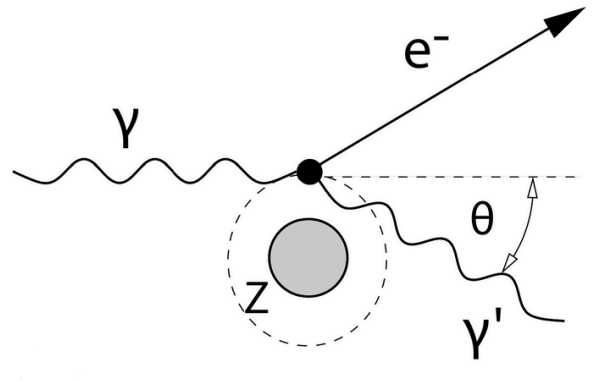
\includegraphics[width =0.4\textwidth]{figures/png/Screenshot_20240812_204345.png}
    \caption[The Compton effect.]{
    The Compton effect \cite{kola}.}
    \label{fig:compt}
\end{figure}

Since the photon scatters quasi-elastically off the electron, 
the energy and angle of the scattered photon are correlated. 
To describe this relationship, we use the 4-momenta defined as 
follows: $k = (E_\gamma, \mathbf{k}c)$ and $p_e = (m_e c^2, 0)$ 
represent the 4-momenta of the photon and the electron (at rest) 
before scattering, and $k' = (E'_\gamma, \mathbf{k}'c)$ and 
$p'_e = (E'_e, \mathbf{p}'_e c)$ represent the 4-momenta 
after scattering. The angle between the scattered photon and 
the incident photon is denoted as $\theta_\gamma$, while the 
angle of the electron is denoted as $\theta_e$. By applying 
energy-momentum conservation:

\begin{equation}\label{compcons}
k + p_e = k' + p'_e
\end{equation}
\begin{equation}\label{compcons2}
(k - k')^2 = (p'_e - p_e)^2 \Rightarrow -k \cdot k' = m_e^2 c^4 - p'_e \cdot p_e
\end{equation}
\begin{equation}
\Rightarrow E_\gamma E'_\gamma (1 - \cos \theta_\gamma) = m_e c^2 \left(E'_e - m_e c^2\right) = m_e c^2 \left(E_\gamma - E'_\gamma \right)
\end{equation}

The right-hand side of the last equation uses the kinetic energy of the electron:

\begin{equation}
T = E'_e - m_e c^2 = E_\gamma - E'_\gamma
\end{equation}

which follows from the energy part of equation \ref{compcons}. 
The energy of the scattered electron as a function of the photon scattering 
angle is derived from equation \ref{compcons2}:

\begin{equation}\label{diffeq}
E'_e = \frac{E_\gamma \cdot \epsilon \cdot (1 - \cos \theta_\gamma)}{1 + \epsilon (1 - \cos \theta_\gamma)}+m_e
\end{equation}

where $\epsilon = \frac{E_\gamma}{m_e c^2}$.

The differential cross section per (free) electron, known as the 
Klein-Nishina formula, is calculated using methods from quantum electrodynamics:

\begin{equation}\label{kleinnishina}
\frac{d\sigma}{d\Omega} = \frac{r_e^2}{2} \frac{1 + \epsilon (1 - \cos \theta_\gamma)}{[1 + \epsilon (1 - \cos \theta_\gamma)]^2} \left(1 + \cos^2 \theta_\gamma + \frac{\epsilon^2 (1 - \cos \theta_\gamma)^2}{1 + \epsilon (1 - \cos \theta_\gamma)} \right)
\end{equation}

An electron bound in an atom can only be considered quasi-free 
if the photon's energy is significantly higher than the electron's 
binding energy. As the photon energy increases, more shell electrons 
become quasi-free, leading to the Compton cross section per atom 
approaching proportionality to $Z$, with individual electrons 
contributing incoherently:

\begin{equation}
\sigma_C^{\text{atom}} = Z\sigma_C
\end{equation}

where $\sigma_C$ is the Klein-Nishina cross section for a 
single free electron. The Compton cross section decreases at 
lower energies, where coherent scattering (Rayleigh scattering) 
off the entire atom (without ionizing the electron shell) becomes dominant.

By reformulating the Klein-Nishina formula, one can obtain the 
differential dependence of the Compton cross section on the 
kinetic energy of the recoil electron $T = E_\gamma - E'_\gamma$:

\begin{equation}
\frac{d\sigma}{dT} = \frac{\pi r_e^2}{m_e c^2 \epsilon^2} \left[2 + \frac{t^2}{\epsilon^2 (1 - t)^2} + \frac{t}{1 - t}\left(t - \frac{2}{\epsilon}\right)\right]
\end{equation}

where $t = T/E_\gamma$. Because the scattering process is 
elastic, there is a one-to-one relationship between the 
energy and angle $\theta_e$ of the electron:

\begin{equation}
\cos \theta_e = \frac{T(E_\gamma + m_e c^2)}{E_\gamma \sqrt{T^2 + 2m_ec^2 T}} = \frac{1 + \epsilon}{\sqrt{\epsilon^2 + 2\epsilon/t}}
\end{equation}

The maximum energy transfer to the electron is obtained 
from equation \ref{diffeq} for backward scattering of the 
photon ($\theta_\gamma = 180^\circ$), corresponding to 
forward scattering of the electron ($\theta_e = 0^\circ$). 
The electron's kinetic energy reaches its maximum value in 
this case, $T \rightarrow T_{\text{max}}$. In the measured 
energy spectrum, this leads to the so-called "Compton edge" at:

\begin{equation}
T_{\text{max}} = \frac{E_\gamma \cdot 2\epsilon}{1 + 2\epsilon}
\end{equation}

which lies slightly below the photopeak. The energy difference 
between the photopeak and the Compton edge $E'_\gamma(\theta = \pi)$ 
decreases with increasing $E_\gamma$ and approaches:

\begin{equation}
E'_\gamma(\theta = \pi) \approx \frac{m_e c^2}{2} \text{ for } E_\gamma \gg m_e c^2
\end{equation}

\subsection{Pair production}
In the Coulomb field of a charge, a photon can 
convert into an electron-positron pair (Figure 
\ref{fig:pprod})\footnote{Photon emission by an 
electron (bremsstrahlung) and pair production are closely 
related processes. By modifying the bremsstrahlung diagram-changing 
the outgoing photon to an incoming one and the incoming electron to 
an outgoing positron-one obtains the pair production 
diagram. The matrix elements of these processes are 
related, at least in the lowest order. Consequently, both 
processes are treated together in the foundational work by 
Bethe and Heitler, often referred to as the 'Bethe-Heitler processes'.}.

\begin{figure}[!h]
    \centering
    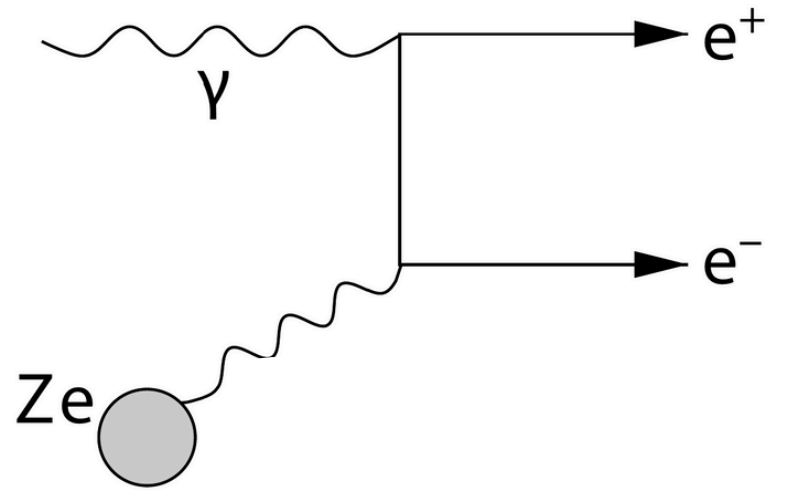
\includegraphics[width=0.4\textwidth]{figures/png/Screenshot_20240812_204755.png}
    \caption[The pair production.]{The pair production \cite{kola}.}
    \label{fig:pprod}
\end{figure}

The energy of the photon must exceed twice the electron 
mass plus the recoil energy transferred to the field-producing 
charge. For most elements, pair production predominantly 
occurs in the Coulomb field of the nucleus. For nuclei, 
the recoil energy is usually negligible, leading to a 
threshold energy for pair production of:
\begin{equation}
    E_{\gamma} \geq 2m_e c^2 + 2 \frac{m_e^2}{m_{\text{nucleus}}} c^2
\end{equation}

If the nuclear charge is not screened by atomic electrons 
(for low energies, the photon must come relatively close to 
the nucleus to make pair production probable, meaning it 
interacts with the "bare" nucleus),
\begin{equation}
    1 \ll \epsilon \ll \frac{1}{\alpha Z^{1/3}}
\end{equation}
the pair-production cross section is given by:

\begin{equation}
    \sigma_{\text{pair}} = 4 \alpha r_e^2 Z^2 \left(\frac{7}{9} \ln 2 \epsilon - \frac{109}{54}\right) \text{ cm}^2/\text{atom}
\end{equation}

However, for complete screening of the nuclear charge ($\epsilon \gg 1/\alpha Z^{1/3}$):
\begin{equation}\label{sigmapair}
    \sigma_{\text{pair}} = 4 \alpha r_e^2 Z^2 \left(\frac{7}{9} \ln \frac{183}{Z^{1/3}} - \frac{1}{54}\right) \text{ cm}^2/\text{atom}
\end{equation}

At high energies, pair production can occur even 
at relatively large impact parameters between the 
photon and the nucleus. In this case, the screening 
effect of atomic electrons must be considered. For 
large photon energies, the pair-production cross 
section approaches an energy-independent value as given by
 Equation \ref{sigmapair}. Ignoring the small term in the equation, 
 the asymptotic value of $1/54$ is expressed as:
\begin{equation}
    \sigma_{\text{pair}} \approx \frac{7}{9} \cdot 4 \alpha r_e^2 Z^2 \ln\left(\frac{183}{Z^{1/3}}\right) \approx \frac{7}{9} \cdot \frac{1}{X_0} \cdot \frac{A}{N_A \rho}
    \label{eq:paircross_radiationlength}
\end{equation}

The energy is uniformly distributed between the produced 
electrons and positrons at low and medium energies, but becomes 
slightly asymmetric at high energies.

The field of the nucleus is formed by the coherent sum of $Z$ 
nucleon charges, leading to the $Z^2$ dependence of the pair 
production cross section.

Even with large momentum transfers $\Delta p$ to the nucleus, 
the energy transfer $(\Delta p)^2/2M$ remains small due to the 
large nuclear mass $M$. After pair creation, the remaining 
energy is equally divided between the $e^+$ and the $e^-$.

\subsection{Delta rays}
High-energy $\delta$-rays, or $knock-on$ electrons, 
are produced when a projectile particle collides 
centrally with shell electrons, resulting in 
significant energy transfers. These electrons 
gain high kinetic energy and can be described 
through elastic collisions with quasi-free electrons. 
By considering the energy-momentum conservation relation 
and using the Lorentz factors $\gamma$ and $\beta$, the 
relationship between the kinetic energy $T$ of the 
$\delta$-ray and the emission angle $\theta$ can be derived as:

\begin{equation}
\cos \theta = \frac{T(\gamma + m_e / M)}{\gamma \beta \sqrt{T^2 + 2T m_e c^2}}
\end{equation}

\begin{equation}
T(\theta) = \frac{2 m_e c^2 \beta^2 \gamma^2 \cos^2 \theta}{\gamma^2(1 - \beta^2 \cos^2 \theta) + 2 \gamma m_e / M + m_e^2 / M^2}
\end{equation}

The maximum energy transfer $T_{\text{max}}$ occurs at $\theta = 0^\circ$, 
while the minimum energy, $T_{\text{min}}$, occurs at $\theta = 90^\circ$. 
At highly relativistic energies ($\gamma \gg 1$ and $\theta \gg 1/\gamma$), 
the energy-angle relationship becomes independent of the incoming particle's properties.

The rate of $\delta$-rays per energy interval $dT$ and path length $dx$ is given by:

\begin{equation}
\frac{d^2 N}{dx \, dT} = n_e \frac{d\sigma}{dT}
\end{equation}

which, when combined with the electron density and the differential cross section, becomes:

\begin{equation}
\frac{d^2 N}{dx \, dT} = \frac{1}{2} z^2 \frac{Z}{A} K \rho \frac{1}{\beta^2} \frac{F(T)}{T^2}
\end{equation}

Here, $K$ is the constant from the Bethe-Bloch formula, 
and $F(T)$ is a function accounting for spin dependence. 
Integration over $T$ and $x$ provides the number of $\delta$-rays in a medium of thickness $\Delta x$:

\begin{equation}
N = \frac{1}{2} z^2 \frac{Z}{A} K \rho \Delta x \frac{1}{\beta^2} \left(\frac{1}{T_{\text{min}}} - \frac{1}{T_{\text{max}}}\right) \approx 0.077 \frac{\text{MeV cm}^2}{\text{g}} z^2 \rho \Delta x \frac{1}{T_{\text{min}}}
\end{equation}

The emission angle dependence is given by:

\begin{equation}
\frac{dT}{d \cos \theta} = 4 m_e c^2 \frac{\cos \theta}{\sin^4 \theta}
\end{equation}

Substituting this into the rate equation yields:

\begin{equation}
\frac{d^2 N}{dx \, d \cos \theta} = \frac{1}{2} z^2 \frac{Z}{A} K \rho \frac{1}{\cos^3 \theta} \frac{1}{m_e c^2} \approx 0.15 \frac{\text{cm}^2}{\text{g}} z^2 \rho \frac{1}{\cos^3 \theta}
\end{equation}

This expression diverges as $\theta$ approaches $90^\circ$, 
where $T$ approaches zero, indicating a limitation in the 
assumption of a free electron. The resulting distributions 
suggest that $\delta$-rays emitted at small angles can 
significantly affect the spatial resolution in detectors, 
particularly through ionization clusters that broaden the 
track of the mother particle.



\section{Monte Carlo samples}\label{datasample}
For our studies, we used three different  
Monte Carlo samples: two samples of 
CE signal generated at two different 
proton pulse intensities, and one sample of 
antiproton annihilation events. 
The production of particles within 
the PT and their tracking from the PS to the 
DS is managed using the Mu2e Offline software 
(Appendix \ref{mu2eana}). The simulation of 
particle interactions is based on 
GEANT4, while the event processing is handled 
by the art framework and data 
management is governed by the SAM system.

The Mu2e simulation uses a technique 
known as multi-stage simulation 
to generate and simulate events efficiently. 
This method involves generating 
events, partially simulating them, and then 
pausing the process to save the 
data generated thus far. Later stages resume 
the simulation from the saved 
state. This approach optimizes both the 
time required for event generation 
and the usage of computing resources. The 
simulation is divided into seven 
stages, S0 through S6, which will be 
briefly discussed in the context of our specific needs:

\begin{itemize}
    \item \textbf{Stage 0}: primary beam protons are generated and propagated 
    inside the PT. When an inelastic interaction occurs at the target, the vertex 
    position is recorded, and the propagation is halted. The probability of 
    inelastic interactions is determined by the total inelastic cross-section 
    ($\sigma_{\text{tot.inelastic}}$) of protons on tungsten (W), which follows the 
    empirical cross section $\sigma_{\text{tot.inelastic}}(\text{W}) = (1710 \pm 30) \ \text{mb}$.
    The probability that a proton from the beam induces an inelastic interaction 
    with the tungsten target is computed using a Monte Carlo approach, that gives 
    $\frac{N_{\text{inelastic}}}{N_{\text{POT}}} = 0.792$. Regarding the generation of $p\bar{p}$ 
    data sample, the number of antiprotons produced per proton on target (POT) at the production target is given by:
    $$
    \frac{N_{\bar{p}}}{POT} = \frac{\sigma_{\bar{p}}}{\sigma_{\text{tot.inelastic}}} \times \frac{N_{\text{inelastic}}}{N_{POT}} = \frac{0.5 \times 0.2824 \, \text{mb}}{1710} \times 0.792 = 6.5 \times 10^{-5}.
    $$
    Antiprotons are generated with a flat momentum distribution between 0 and 5 GeV/c and 
    are assumed to have isotropic directions;
    
    \item \textbf{Stage 1}: events are propagated through the TS and PS. 
    Only those particles that reach a virtual detector (VD) in front 
    of the TS entrance are saved as input for the next stage;

    \item \textbf{Stage 2}: in this stage, $\pi^-$, $\mu^-$, and $\bar{p}$ 
    particles are stored and tracked. To enhance statistics, a resample factor 
    is applied here: each $\bar{p}$ from S1 is traced multiple times, creating 
    independent events due to statistical fluctuations in energy losses within 
    the absorbers. A resample factor of $10^5$ keeps oversampling under control;

    \item \textbf{Stage 3}: particle transportation from the COL3u exit to the TS5 entrance;

    \item \textbf{Stage 4}: particle transportation from TS5 to the ST, 
    where the positions of stopped pions and muons are stored;

    \item \textbf{Stage 5}: to optimize simulation efficiency, $3 \cdot 10^7$ 
    stationary pions and antiprotons are generated at rest at the stopping 
    target, using the recorded time and position of the stops. These particles 
    are then propagated to the detectors. For the CE dataset, a fraction of muons 
    are assumed to decay into conversion electrons. For the $\bar{p}$ dataset, 
    antiproton annihilation at rest in the ST is simulated based on the positions 
    and times of the stopped antiprotons. Background electrons from annihilation 
    result from decays such as $\pi^0 \to \gamma \gamma$, followed by photon 
    conversions, and $\pi^- \to \mu^- \nu$, followed by $\mu^-$ decays. During 
    this stage, the raw simulated data are digitized into simple C++ classes or 
    structs, mimicking the detector's raw data;

    \item \textbf{Stage 6}: Finally, reconstruction from detector hits is performed.
\end{itemize}

Regarding CPU time, Stages 0 and 1 are the most time-consuming. 
Stage 2 can also be demanding when a high resampling factor is used, 
while the later stages are significantly faster by an order of magnitude.

A typical Mu2e event includes multiple hits from particles produced 
by muon captures in the ST, as well as particles entering the DS from 
the TS. These hits are called pileup hits, which make 
up the majority of the detector's hits. The pileup level 
depends on the proton pulse intensity. The Mu2e pileup 
simulation assumes that the pulse intensity varies on a 
time scale much longer than 2 $\mu$s, meaning all proton 
pulses around the simulated one share the same intensity. 
Under this assumption, a transformation is applied to hits 
with time $T_i > 1695$ ns outside the microbunch limits, 
assigning them a new time $t_i = \frac{T_i}{1695}$ ns, 
effectively accounting for late hits that would otherwise 
be attributed to later microbunches. 

For low-intensity mode, with a mean intensity of 
$1.6 \times 10^7$ protons/pulse, which in Mu2e 
jargon is named "1BB", approximately 25,000 
muons stop in the ST per pulse. In the high-intensity 
mode, named "2BB", this number is about 2.5 times higher (Section \ref{pulsedprotonbeam}).

The datasets used for CE signal plus pileup 
analysis will be referred to as $CE-1BB$ and $CE-2BB$ 
for 1BB and 2BB pileup, respectively. The dataset for 
antiproton analysis without pileup will be 
referred to as $PBAR-0BB$.
For datasets with pileup, 
the pileup hits are explicitly added to the hits from 
the signal process. In the antiproton sample, however, 
no pileup hits are added, meaning the data represents 
pure antiproton sample. 
\section{$\delta$-electrons in the Mu2e tracker}

In Mu2e, low-energy electrons 
and positrons, with a momentum below 20 MeV/c and 
referred to as $\delta$-electrons, 
generate the majority of hits in the tracker. 
Identifying the $\delta$-electrons hits as early 
as possible would be crucial to optimize memory 
and CPU usage. There are also several physics 
reasons why it would be important to identify 
those hits correctly:
\begin{itemize}
    \item the main Mu2e goal is the search for the 
    CE signal: flagging erroneously even a small 
    fraction of the hits generated by the 
    CE as $\delta$-electrons may result in a 
    reduction of the CE track reconstruction efficiency. 
    Figure \ref{fig:momhits} shows that in the 
    Monte Carlo sample $CE-1BB$, the simulated CE 
    hits are just 1\% of the total hits in the tracker;
    \item counting the number of protons 
    will be a complementary procedure to the 
    STM to determine the muon stopping rate: 
    the simulation shows that is possible to 
    estimate the number of muons captured in 
    the stopping target by counting the number 
    of protons produced in the nuclear muon 
    capture, which has a probability of 61\%.    
    \item the misidentification of muons 
    and pions as protons or $\delta$-electrons 
    may result in errouneous background estimate. 
    This is particularly significant for the 
    antiproton background.
    $p\bar{p}$ annihilation at rest in the ST 
    can produce signal-like electrons, which 
    constitute a background to the CE search, 
    but the estimate for this background is 
    presently affected by a large systematic 
    uncertainty. Mu2e has developed a data-driven 
    procedure to improve the estimate.
    $p\bar{p}$ annihilation at rest in the ST 
    can produce events with two or more tracks, 
    each with a momentum around 100-200 MeV/c. 
    For $p\bar{p}$ annihilation, 
    the rate of multi-track events 
    is about 500 times higher 
    than the rate of events with a single 
    signal-like electron. 
    For $10^4$ $p\bar{p}$ annihilation events 
    generated, about 3.7\% of 
    the events contained two reconstructable 
    particle tracks. Therefore, 
    the identification and reconstruction of 
    multi-track events could be 
    used to constrain the $p\bar{p}$ background. 
    Thus, it is crucial not to flag hits 
    generated by muons or pions as $\delta$-electron 
    hits, since this would compromise the 
    reconstruction efficiency. 
\end{itemize}
Figure \ref{fig:momhits} shows the 
momentum distribution (Monte Carlo truth) of 
particles that make at least one hit in the 
tracker for a simulated CE sample ($CE-1BB$, 
Section \ref{datasample}). 
For each Monte Carlo particle, the 
histogram is filled a number of times 
equal to the number of hits generated 
by that particle.
The distribution shows that the 
majority of hits originate from 
low-energy electrons and positrons 
(orange), which constitute approximately 
75\% of the total number of hits. 
There is an asymmetry between the 
number of hits below 20 MeV/c 
produced by electrons and positrons: 
electrons account for 
71\% of all $\delta$-electron hits in 
the tracker, while positrons 
contribute only 4\%. This discrepancy 
arises because only electrons 
undergo Compton scattering, which is 
the primary source of hits in the energy 
range of 1 MeV. This difference 
will be crucial in 
the following sections when discussing 
the $\delta$ flagging efficiency.

The distribution also shows that 14\% of 
the total hits are due to protons, 
which are produced by nuclear processes. 
In particular, the first peak in proton  
momentum distribution is due to  
inelastic neutron scattering, while 
larger momentum values correspond muon 
capture at rest.
Their kinetic energy ranges from about 
5 to 20 MeV, resulting in low $\beta \gamma$ values, 
which makes them heavily ionizing particles. 
The deposited energy will be 
one of the variables used to discriminate protons. 

It is important to note that the bump 
around 50 MeV/c in 
the positron distribution should not be 
present. According 
to the Monte Carlo truth, this is due to 
muon Decay-In-Flight, 
and we expect 
$N(\mu^+ \rightarrow e^+ )/N(\mu^- \rightarrow e^- )$ 
to be about $10^{-3}$ 
for muons entering the DS. The DIO on the IPA 
(Section \ref{detectorsolenoid}) 
should also be around 
$10^{-3}$ compared to the DIF of 
negative muons. 
The simulation of $\mu^+$ may 
contain some errors and we are still 
investigating this discrepancy. 
However, this issue is not problematic for the analysis 
of low-momentum electrons and positrons, 
as the momentum ranges are different.

\begin{figure}[!h]
        \centering
        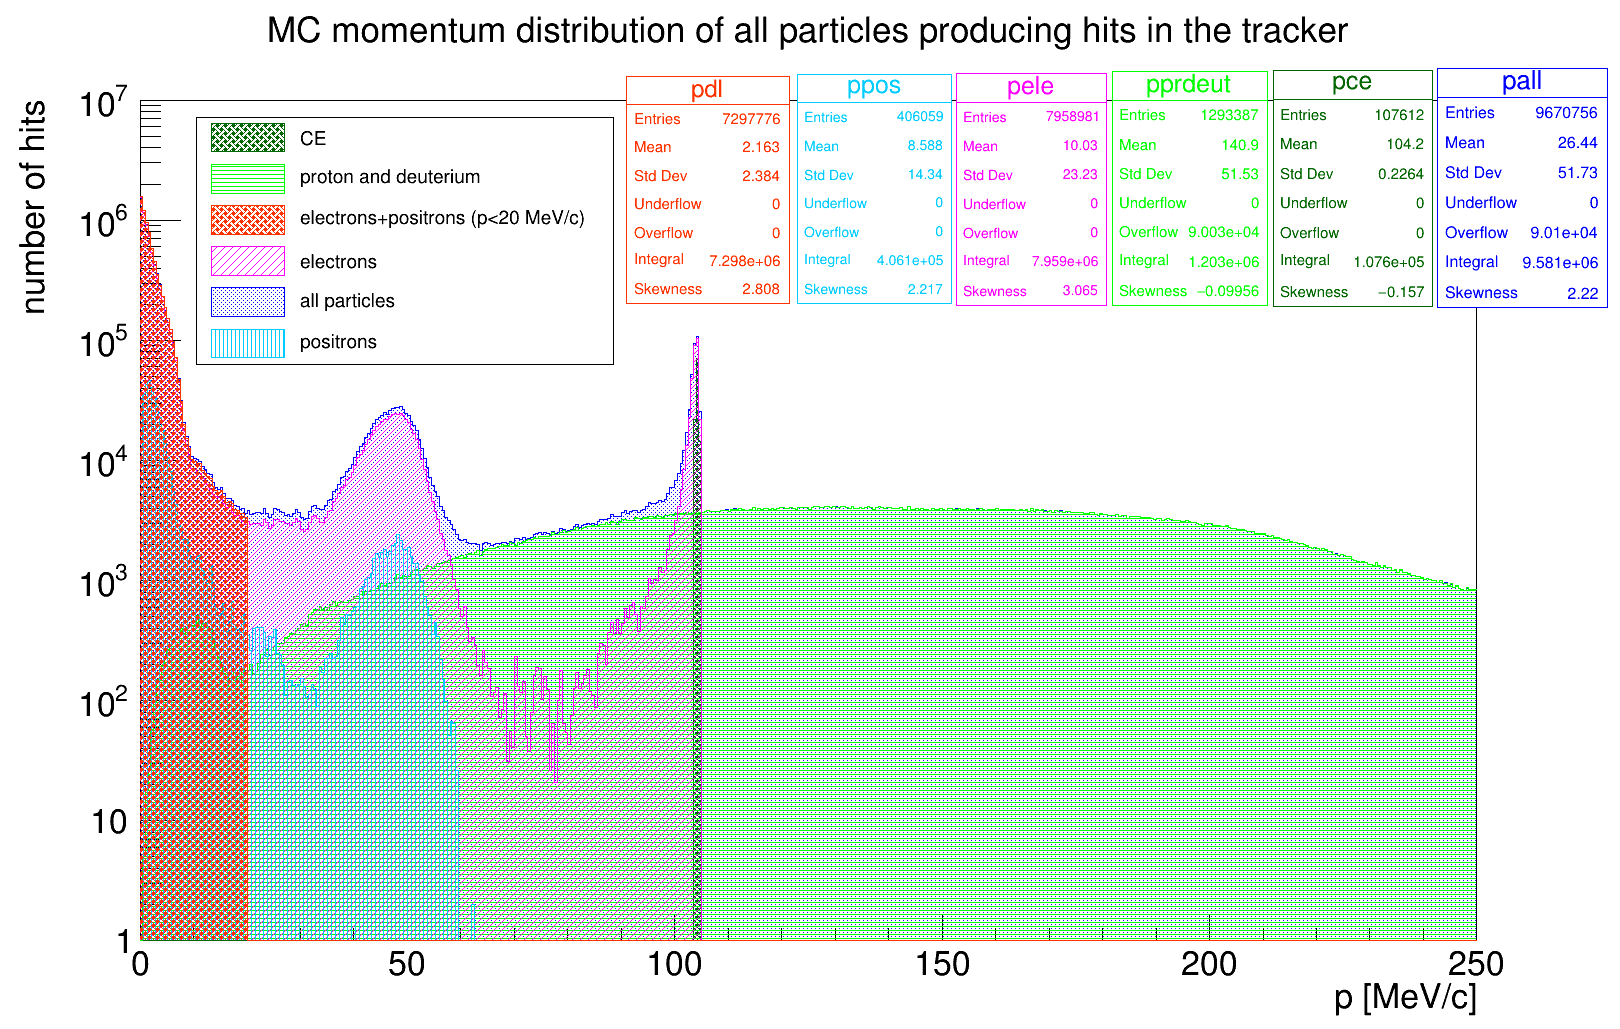
\includegraphics[width =0.95\textwidth]{figures/png/Screenshot_20240812_152905.png}
    \caption[Monte Carlo momentum distribution 
    of particles producing hits in the Mu2e 
    tracker ($CE-1BB$ data sample).]{
        Momentum distribution (Monte Carlo truth)  
       of particles producing at 
       least one hit in the tracker 
       ($CE-1BB$ data sample).  
       The momentum distribution 
       of all particles making hits is 
       depicted in dark blue, with electrons 
       shown in pink, positrons in light 
       blue, $\delta$s in orange, protons 
       and deuterons in 
       light green, and CEs in dark green. }
       \label{fig:momhits}
\end{figure}


Figure \ref{fig:pbar} shows the true 
momentum distribution of 
particles produced in the $p\bar{p}$ 
annihilation at the ST. 
The data sample ($PBAR-0BB$) is described in Section \ref{datasample}.
For each Monte Carlo particle, the histogram 
is filled a number of times equal to the number 
of hits generated by that particle. 
The particles produced in the $p\bar{p}$ annihilation 
are mostly pions, muons, and a few electrons. 
The momentum distribution has a 
peak in the 100-200 MeV/c range. Photons are also 
produced, and they can undergo Compton scattering and 
pair production, which explains the presence of a 
$\delta$-electron peak that is about $\sim$100 
times lower than the one in Figure \ref{fig:momhits}.

\begin{figure}[!h]
    \centering
    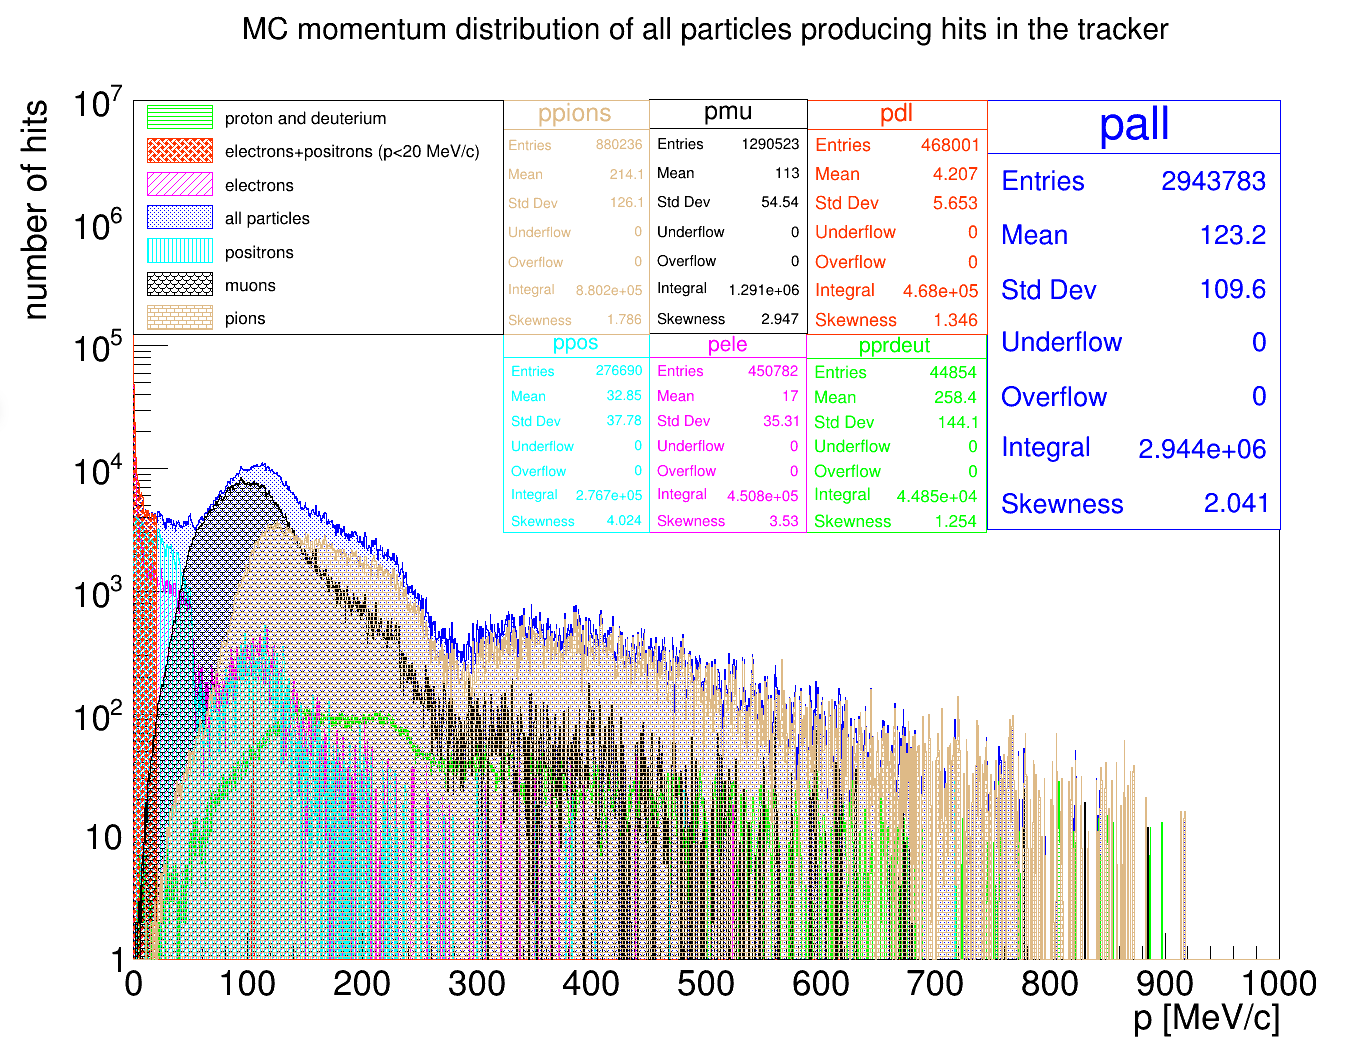
\includegraphics[width =0.9\textwidth]{figures/png/Screenshot_20240815_124710.png}
\caption[Monte Carlo momentum distribution 
of particles producing hits in the Mu2e 
tracker ($PBAR-0BB$ data sample).]{
    Momentum distribution (Monte Carlo truth) 
    of particles producing at 
   least one hit in the tracker 
   ($PBAR-0BB$ data sample). 
   The momentum distribution 
   of all particles making hits is 
   depicted in dark blue, with electrons 
   shown in pink, positrons in light 
   blue, $\delta$s in orange, protons 
   and deuterons in green, pions in 
   light brown and muons 
   in black. }
   \label{fig:pbar}
\end{figure}
Figure \ref{fig:momhits} shows that 
the majority of the recorded hits 
originate from $\delta$-electrons, 
with protons being the second most 
common source. Figure \ref{fig:afbef} 
presents an example of comparison of an 
event display before and after the background 
hits have been flagged and removed.  
Flagging these hits is crucial for 
several reasons: it prevents unnecessary 
data from being sent to the pattern 
recognition algorithms, thereby conserving 
CPU resources and reducing processing 
time. Moreover, it is important to avoid 
storing these hits on tape, as doing so 
would lead to inefficiencies in data storage.

\begin{figure}[!h]
    \begin{subfigure}[b]{0.4\linewidth}
        \centering
        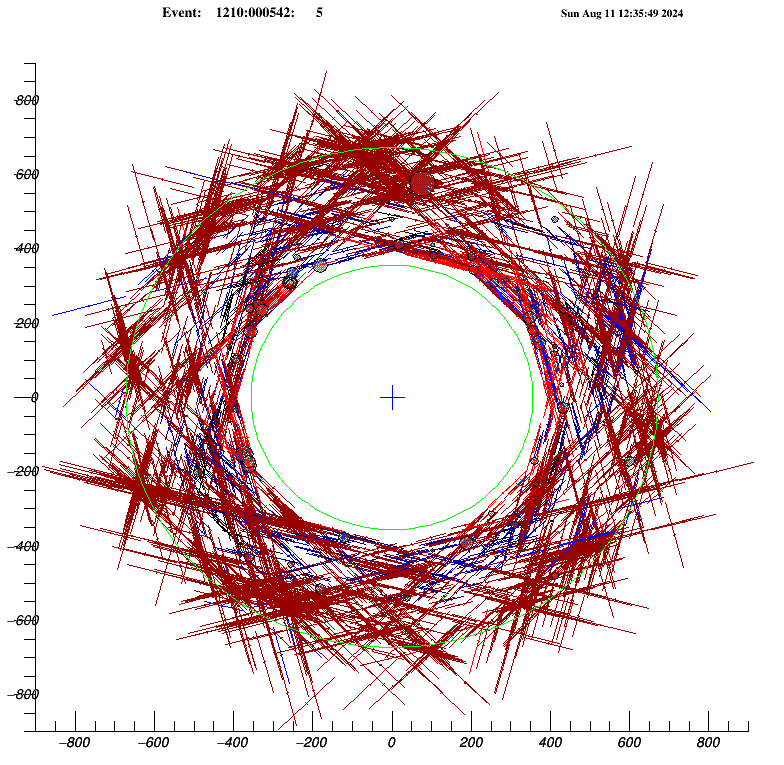
\includegraphics[scale = 0.3]{figures/png/Screenshot_20240811_123612.png}
        \subcaption{Before.}
        \label{fig:bef}
    \end{subfigure}
    \begin{subfigure}[b]{0.7\linewidth}
        \centering
        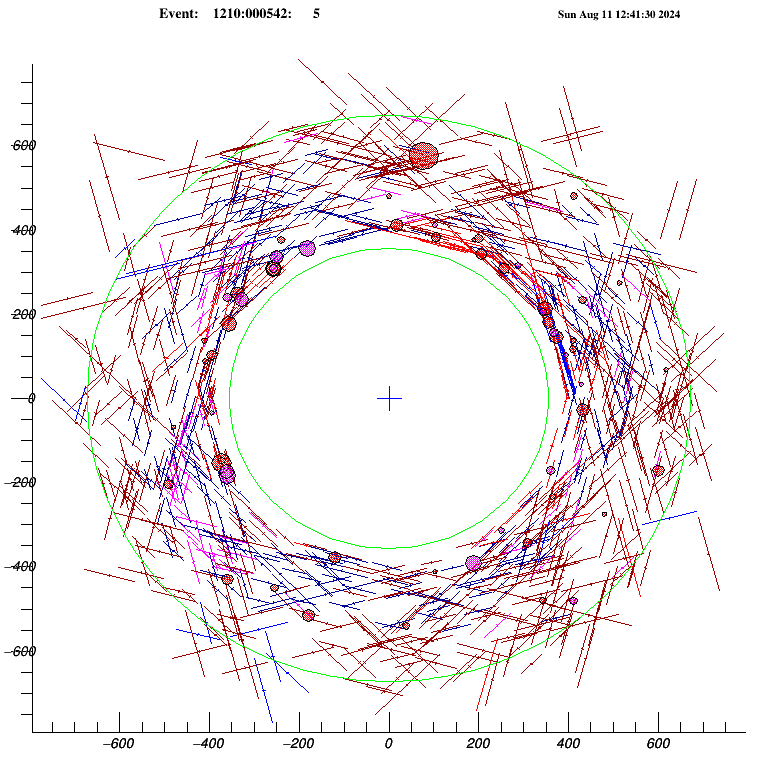
\includegraphics[scale = 0.3]{figures/png/Screenshot_20240811_124245.png}
        \subcaption{After.}
        \label{fig:af}
    \end{subfigure}
    \caption[Before and After background hits flagging.]{
        Before and After background hits flagging. 
        The $x-y$ plane views of a CE 
    event with 2BB pile-up in the tracker (Section \ref{pulsedprotonbeam}). 
    The segments are the $hit$ tracker straws. 
    The hits marked in
    red are from electrons and the ones in 
    blue are from positrons. Left (Right): before (after) $\delta$-electron hit flagging.}
    \label{fig:afbef} 
\end{figure}






\section{$\delta$-electrons flagging algorithms}
A description of the Mu2e Offline software 
tool is reported in 
Appendix \ref{mu2eana}, and the reconstruction 
process is described in Appendix \ref{eventreco}. 

Flagging $\delta$-electrons is a major early 
step in the Mu2e reconstruction  
and it is executed before time clustering 
and pattern recognition.

Mu2e has developed two types of flagging algorithms:
\begin{itemize}
    \item $FlagBkgHits$, described in Section \ref{flagbkghits};
    \item $DeltaFinder$, described in Section \ref{deltafinder}.
\end{itemize}

\subsection{The $FlagBkgHits$ algorithm}\label{flagbkghits}
The detailed description of multivariate 
analysis (MVA) and the 
process of MVA training are beyond the 
scope of this work. 
Nevertheless, since this technique is 
one of the options 
developed for background flagging, I 
will briefly outline 
the fundamental principles involved.

When searching for patterns in a multivariable space, 
a common procedure involves 
defining a set of statistical 
models that analyze the measured 
variables and estimate 
the probability that these are consistent with the 
sought pattern. Once the variables are selected, 
the MVA is trained to recognize patterns by 
evaluating examples known to the trainer, 
allowing for feedback to refine the 
pattern identification procedure.

The first selection concerns the 
mean energy deposited in  
the $ComboHit$s used to create a 
$StereoHit$ and excludes 
those with a deposited energy above 5 keV. 
The algorithm then classifies as 
protons all hits with a deposited 
energy above 4.5 keV.
Other selections concern the timing, 
position, and spread of the $ComboHit$ 
in the $x$-$y$ plane. The maximum cluster timing 
and diameter are 20 ns and 5 mm, respectively.

Since $\delta$-electrons tend to form small, dense 
clusters of hits on $x$-$y$ plane, an algorithm based on a clustering 
approach was developed: concentrated clusters in the 
$x$-$y$ plane are sought using a clustering algorithm, 
as $\delta$-electrons are highly likely to reside 
in such clusters. The $FlagBkgHits$ algorithm uses  
a hit-level MVA to ensure that hits within a 
$\delta$-dominant cluster truly belong there, 
and a cluster-level MVA to differentiate 
$\delta$-dominant clusters from those 
predominantly containing CEs. 
This was trained in a supervised mode, 
using CE and $\delta$-electrons hits from 
Monte Carlo data sample.

The resolution on the measurement of the 
hit position performed by the straw drift 
tube is limited to a few cm. 
However, an improved position measurement can be 
achieved by leveraging the multiple straw layers that 
significantly overlap in the $x-y$ plane. 
By obtaining two hit measurements from a pair of 
intersecting straws and ensuring they fall within 
a time window on the order of the maximum drift time, 
one can deduce that these hits were produced by the 
same particle and occurred at the intersection of the 
two straws in the $x-y$ plane. This method, 
involving two-dimensional information from the two 
straws, is referred to as the stereo information method.

The clustering process uses the $x$ and $y$ coordinates 
of the selected hits. A random hit is chosen to define 
the initial cluster, after which the following iterative 
steps are applied. The centroid of each cluster is 
computed, and hits whose distances from a cluster 
centroid fall within a specified inner threshold 
and time window are added to that cluster. Hits 
with distances from all existing clusters greater 
than an outer threshold are used to seed new 
clusters, while hits that fall between the two 
thresholds remain unassigned. This process 
generates a new set of clusters, preparing the 
system for the next iteration. During each 
iteration, every hit is reconsidered as a 
potential new point in a cluster, including 
those already assigned. The clustering process 
continues until convergence is achieved, i.e., 
when an iteration no longer results in any changes.


\subsection{The $DeltaFinder$ algorithm}\label{deltafinder}

The $DeltaFinder$ algorithm has been designed 
to identify $\delta$-electron 
hit patterns rather than CE hits. This 
algorithm relies on the 
fact that $\delta$-electrons typically 
form a straight line in 
the $r$-$z$ plane (cyan lines in Figure 
\ref{fig:yzviewdelta}) 
and appear as a spot with a diameter 
of less than $\sim$3 cm in the 
$x$-$y$ plane within the 1 T  
magnetic field. On the other hand, 
CEs create entirely different 
patterns of hits, which appear as oblique segments in 
the $r$-$z$ plane due to their 
helical trajectories (red lines 
in Figure \ref{fig:yzviewdelta}). 
\begin{figure}[!h]
    \centering
    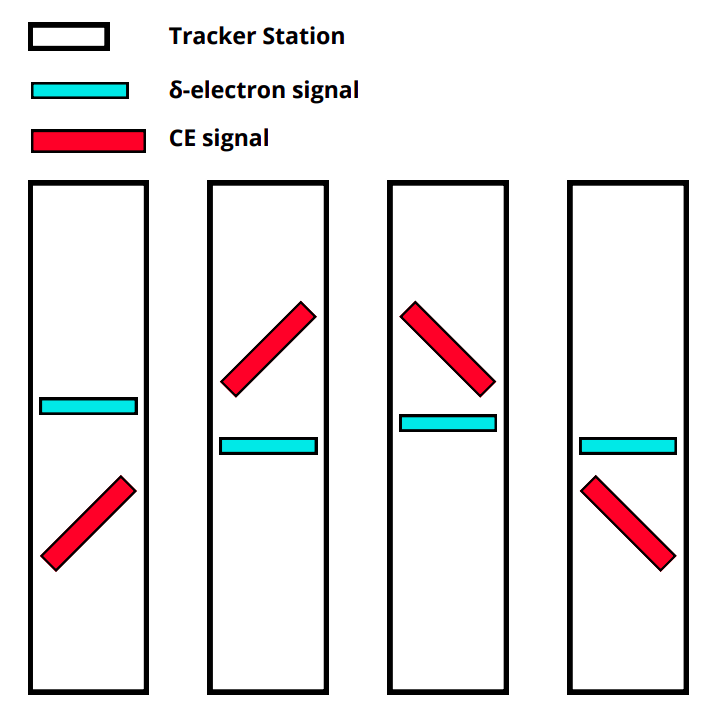
\includegraphics[width =0.6\textwidth]{figures/png/Screenshot_20240811_123048.png}
    \caption[$\delta$-electrons and CE patterns in $r-z$ plane.]{
        $\delta$-electrons and CE patterns in the $r-z$ plane. 
        The white rectangles represent four of the eighteen tracker stations. 
        The cyan straight lines represent a possible $\delta$-electron 
        patterns, while the red lines a possible CE pattern.
        }
    \label{fig:yzviewdelta}
\end{figure}
\subsubsection{Step 1: identifying $\delta$-electron segments}
The $DeltaFinder$ first tries to 
identify $\delta$-electron track 
segments within each station 
individually. These segments, 
parallel to the beam axis, are 
called $seeds$. Since hits 
from the same electron should be 
close in both time and space, 
and $\delta$-electrons may hit 
multiple straws within the 
same panel, the algorithm clusters 
these straw hits in 
in space and time, applying various 
cleanup cuts to ensure the 
selected patterns resemble 
$\delta$-electron hits. 
The maximum allowed time 
difference between two hits within 
a station to form a $seed$ is set to 40 ns.

These cleanups based on the $x$-$y$ 
coordinates are performed 
by computing a $\chi^2$. The $seed$ 
is reconstructed using 
two, three, or four $ComboHit$s. 
In each case, the 
intersections between two straws 
are determined, 
and the $x$-$y$ coordinates of 
the $seed$ are given 
by the center of gravity of 
these intersections. 
In the case of only two hits, 
the center of gravity 
corresponds to the stereo hit. 

The algorithm extends the $seed$s by requiring 
hits to be sufficiently close to the intersection 
point in time and space, performing multiple checks 
to avoid over-efficiency in 
hit flagging. For each $seed$, 
the mean deposited energy is calculated from the energy 
deposited in all $ComboHit$s. Based on the mean 
deposited energy of a $seed$ in a station, hits with 
energy above 5 keV are considered proton hits. 
This selection optimizes data processing by 
reducing the total number of hits that need to be analyzed.

\begin{figure}[!h]
    \centering
    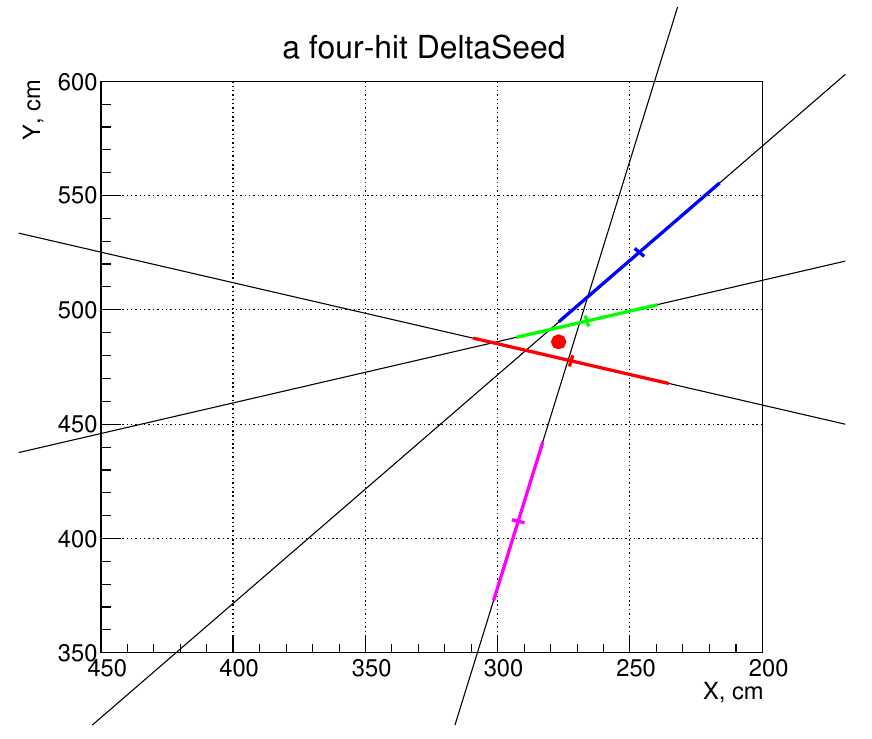
\includegraphics[width =0.6\textwidth]{figures/png/Screenshot_20240811_115854.png}
    \caption[A $\delta$ candidate $seed$.]{A 
    $\delta$ candidate $seed$. The four 
    coloured segments are the tracker straws that were
    hit in the same station.}
    \label{fig:deltaseeds}
\end{figure}

It is necessary clarify one detail. 
Figure \ref{fig:energydeposited} shows the 
distribution of the simulated deposited energy 
in the tracker for $\delta$ electrons, CEs, and 
protons in the case of a 1BB pileup. 

To optimize data processing, a hit energy 
threshold could be applied to the $DeltaFinder$ 
to reduce the total number of hits that 
need to be analyzed, 
thereby speeding up the process. Moreover, only about 
4\% of CE hits have energies above 3.5 keV 
(and 1\% above 5 keV), so the loss of CE 
hits would be minimal, resulting in a 
faster overall algorithm. 

However, implementing such an energy cutoff has a 
significant impact for the algorithm's performance. 
Starting with fewer hits, especially in 
stereo intersections, 
reduces the likelihood of 
identifying the correct $seed$. 
Moreover, a higher energy cutoff increases 
the probability of false positives, as the algorithm 
aims to count protons too.

\begin{figure}[!h]
    \centering
    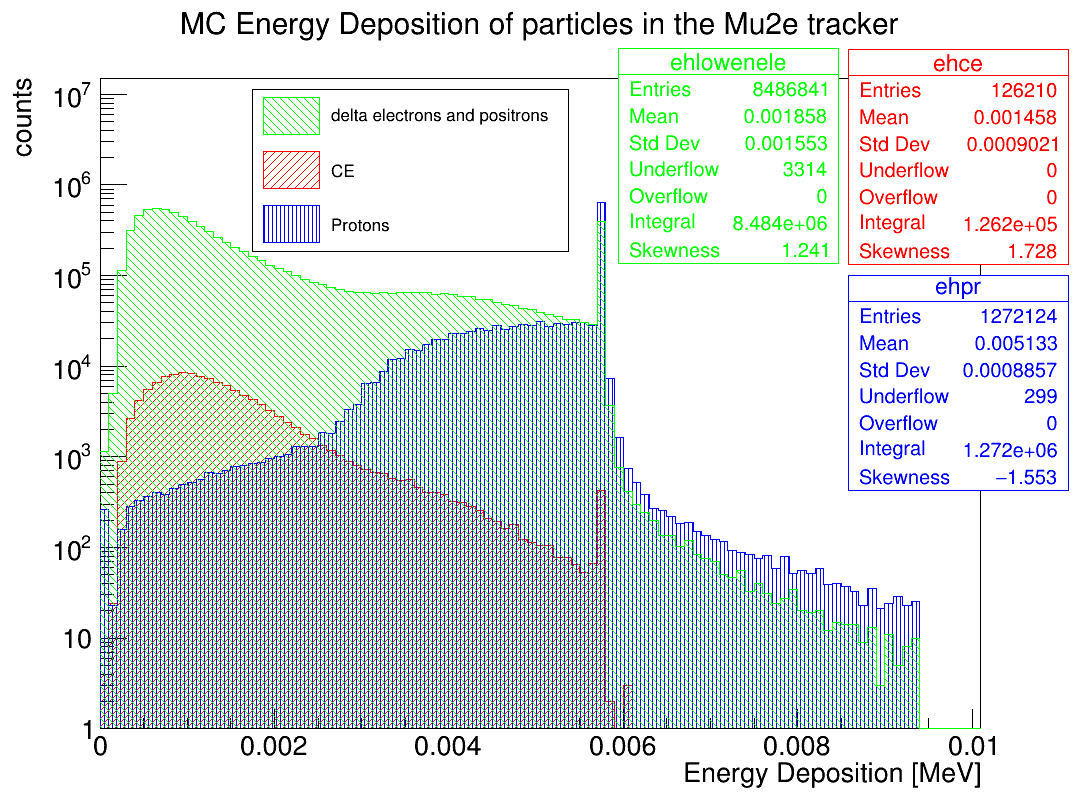
\includegraphics[width =0.6\textwidth]{figures/png/Screenshot_20240729_151910.png}
\caption[Monte Carlo deposited energy 
distribution in the tracker.]{
   The Monte Carlo deposited energy 
   distribution in the tracker ($CE-1BB$ data sample).  
   The red distribution refers to 
   CEs, while the 
   green and the blue one to $\delta$-electrons 
   and protons respectively. 
   The peaks and tails correspond to 
   particles with such high energy 
   deposition that they result in a 
   saturated waveform.

}
   \label{fig:energydeposited}
\end{figure}
\subsubsection{Step 2: connecting $seed$s}
After the selection based on mean deposited energy, 
$DeltaFinder$ attempts to connect segments that 
are close in both the $x$-$y$ plane and time 
across different stations to form $\delta$-electron 
candidates. A valid candidate must have at 
least two segments and a minimum of five straw hits. 
Reconstructed segments from a 100 MeV electron 
typically remain unconnected due 
to their separation in the $x$-$y$ plane. 

$DeltaFinder$ links $\delta$-electron $seed$s 
across stations, attempting to associate new $seed$s 
with existing $\delta$ candidates. If no match is 
found, a new candidate is created. Good $\delta$ 
candidates are marked, and their hits are 
flagged to prevent their inclusion in proton candidate searches.

\subsubsection{Step 3: Identifying Proton Candidates}
Finally, $DeltaFinder$ identifies proton candidates 
using the remaining $seed$s, which are more likely 
to have deposited energy above 3 keV. First, it checks 
if a $seed$ is consistent in time with any existing 
proton candidate. If no consistency is found, 
the hits of the $seed$ are added to a new proton candidate.


\section{Performance analysis and comparison between $FlagBkgHits$ and $DeltaFinder$}
The comparison between $FlagBkgHits$ and $DeltaFinder$ 
is performed at two levels of 
comparison, with each level addressing different aspects 
of the algorithms:

\begin{itemize}
    \item \textbf{Hit-level comparison}: this phase focuses 
    on evaluating how accurately individual hits are 
    flagged, providing the most direct method for 
    assessing and comparing the performance of the two 
    algorithms. This stage allows for an unbiased 
    comparison without the influence of subsequent 
    reconstruction stages. It also includes a direct evaluation of proton counting;
    
    \item \textbf{High-level comparison}: this phase examines 
    the algorithms' impact on the later stages of 
    event reconstruction. It highlights how effectively 
    each algorithm contributes to the accurate reconstruction 
    of tracks. The main figure of merit at this stage is the 
    reconstruction of CE tracks, as well as the background reconstruction.
\end{itemize}

\subsection{Hit-level comparison}
Before starting with the hit-level comparison of the two algorithms, during the analysis, 
we first observed an over-efficiency in the proton hit flagging by $DeltaFinder$. 
This primarily impacted the flagging of protons, muons, and pions, as shown in 
Table \ref{tab:1bbcelebefore} and Table \ref{tab:0bbpbarbefore}. In these tables 
and the ones that follow, $f_p$ and $f_e$ represent 
the number of $ComboHit$s flagged as protons and electrons, respectively, 
divided by the total number of $ComboHit$s. DF and FBH denote the $DeltaFinder$ 
algorithm and $FlagBkgHits$, respectively. Each row corresponds to the particle 
under study.
\begin{center}
    \begin{table}[h!]
    \centering
    \renewcommand{\arraystretch}{1.}
    \begin{tabular}{| c | c | c |} 
    \hline
    & $f_{p}$ & $f_{e}$ \\
    \hline
    $p$     & 96.0\% & 1.0\% \\
    \hline
    \end{tabular}
    \caption[$DeltaFinder$ proton 
    flagging results before the adjustment.]{$DeltaFinder$ proton 
    flagging results before the 
    adjustment ($CE-1BB$ data sample). 
    $f_p$ and $f_e$ represent 
    the number of proton $ComboHit$s 
    flagged as protons and electrons, respectively, 
    divided by the total number of $ComboHit$s.}
    \end{table}\label{tab:1bbcelebefore}
\end{center}
    
\begin{center}
    \begin{table}[h!]
        \centering
        \renewcommand{\arraystretch}{1.}
        \begin{tabular}{| c | c | c | c | c|} 
        \hline
        &   $f_{p}$ &   $f_{e}$\\
        \hline
        $\mu$ &  5.8\%  & 5.0\%\\
        \hline
        $\pi$ & 2.5\% &  11.2\%\\
        \hline
        \end{tabular}
        \caption[$DeltaFinder$ muon and 
        pion flagging results before the adjustment.]{$DeltaFinder$ muon 
        and pion flagging results before the adjustment ($PBAR-0BB$ data sample). $f_p$ and $f_e$ represent 
        the number of particle $ComboHit$s flagged as protons and electrons, respectively, 
        divided by the total number of $ComboHit$s.}
    \end{table}\label{tab:0bbpbarbefore}
\end{center}

The number of pions and muons flagged as protons is extremely high. 
Figure \ref{fig:0pbarbefore} shows the distribution of the total 
number of muon $ComboHit$s (red) and those flagged as $\delta$s (blue) 
and protons (green) versus the particle momentum. 
As shown, a significant number of muons were misidentified 
as protons when the momentum was low. 
According to the Bethe-Bloch formula, such hits have 
higher energy loss and can thus be most likely flagged as 
protons. Upon realizing this issue, we made slight modifications to the 
algorithm. Since $seed$s may have accidentally attached hits, we imposed a 
condition requiring a $good$ proton candidate to have more than four 
hits with a deposited energy greater than 3 keV.

This adjustment is slightly inefficient for protons, reducing their 
efficiency by a 10\% (Tables \ref{tab:1bbcele} and \ref{tab:2bbcele}). 
However, it significantly reduces the 
number of muons and pions flagged as protons, by approximately 
a factor of 2 and a factor of 6 (Table \ref{tab:0bbpbar}), respectively.

 \begin{figure}[!h]
            \centering
            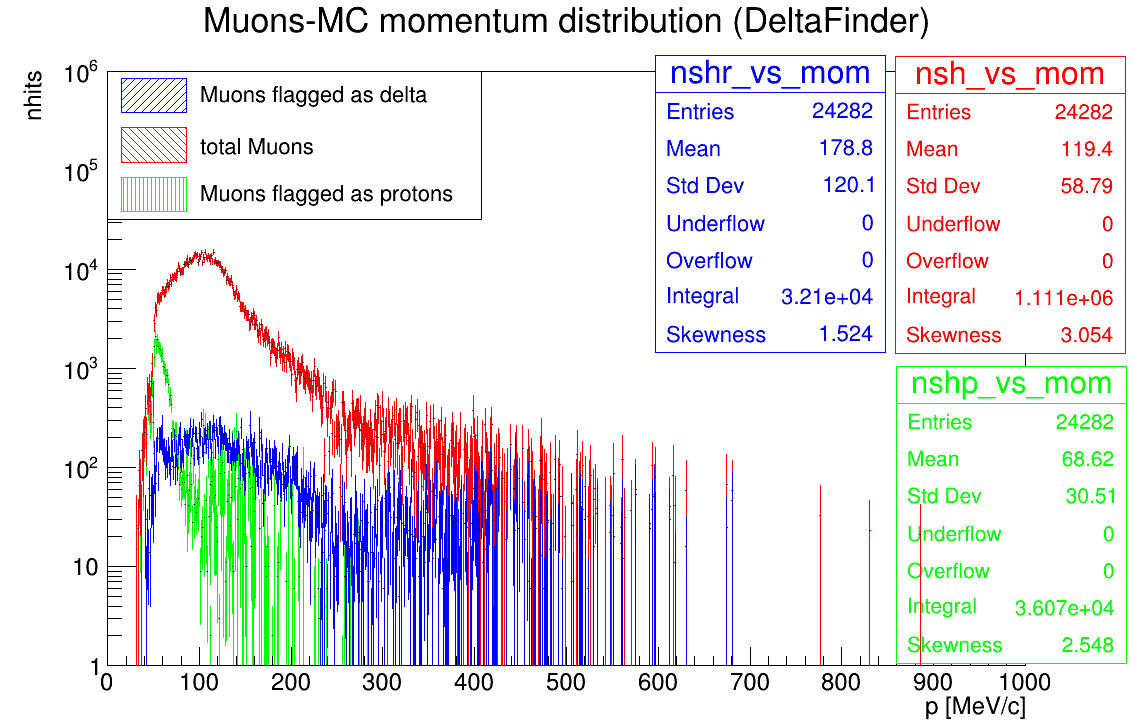
\includegraphics[width =0.7\textwidth]{figures/png/Screenshot_20240805_222923.png}
        \caption[The momentum 
        distribution of the total 
        and flagged number of muon 
        $ComboHit$s.]{The momentum 
        distribution of the total number of 
        muon $ComboHit$s 
        (red) and of the muon $ComboHit$s 
        flagged as $\delta$s (blue) 
        and protons (green) ($PBAR-0BB$ data sample). }
           \label{fig:0pbarbefore}
\end{figure}

Now let's move on to the performance analysis and comparison part.

Tables \ref{tab:2bbcele} and \ref{tab:1bbcele} show the hit-level 
comparison for the $CE-1BB$ and $CE-2BB$ data samples between the two algorithms.
\begin{center}
    \begin{table}[h!]
    \centering
    \renewcommand{\arraystretch}{1.}
    \begin{tabular}{| c | c | c | c |} 
    \hline
    &    $f_{p}$ DF & $f_{e}$ FBH  & $f_{e}$ DF \\
    \hline
    e$^-$ ($p<$20 MeV/c)      & 3.7\%   & 75.1\% & 72.7\%\\
    \hline
    e$^-$ (20$<p<$80 MeV/c)  & 2.2\%   & 49.0\%& 29.9\%\\
    \hline
    e$^-$ (80$<p<$110 MeV/c)  & 0.8\%  &  7.4\%& 4.3\%\\
    \hline
    $p$       &  83.6\%  &  & 2.2\%\\
    \hline
    e$^+$ ($p<$20 MeV/c) & 0.4\%    &   84.2\%& 87.9\%\\
    \hline
    \end{tabular}
    \caption[Electrons, 
    positrons and protons hit-level comparison.]{Electrons, 
    positrons and protons hit-level comparison ($CE-2BB$ data sample). FBH and DF denote  
    the $FlagBkgHits$ and the $DeltaFinder$ algorithms, respectively. $f_p$ and $f_e$ represent 
    the number of particle $ComboHit$s flagged as protons and electrons, respectively, 
    divided by the total number of $ComboHit$s.
    }
    \end{table}\label{tab:2bbcele}
    \end{center}

    \begin{center}
    \begin{table}[h!]
    \centering
    \renewcommand{\arraystretch}{1.}
    \begin{tabular}{| c | c | c | c |} 
    \hline
   &  $f_{p}$ DF & $f_{e}$ FBH  & $f_{e}$ DF \\
    \hline
    e$^-$ ($p<$20 MeV/c)     & 2.5\%   & 75.9\% & 72.5\%\\
    \hline
    e$^-$ (20$<p<$80 MeV/c)  & 1.0\%   & 50.0\%& 27.4\%\\
    \hline
    e$^-$ (80$<p<$110 MeV/c)   & 0.3\%  &  5.7\%& 3.4\%\\
    \hline
    $p$                 &         83.7\%   &  & 1.0\%\\
    \hline
    e$^+$ ($p<$20 MeV/c)    & 0.2\%    &   85.5\%& 88.5\%\\
    \hline
    \end{tabular}
    \caption[Electrons, positrons and protons hit-level comparison.]{Electrons, 
    positrons and protons hit-level comparison ($CE-1BB$ data sample). 
    FBH and DF denote the $FlagBkgHits$ and the $DeltaFinder$ 
    algorithms, respectively. $f_p$ and $f_e$ represent 
    the number of particle $ComboHit$s flagged as protons and electrons, respectively, 
    divided by the total number of $ComboHit$s.}
    \end{table}\label{tab:1bbcele}
    \end{center}
  
The fraction of electrons and positrons flagged as $\delta$-electrons 
differs due to the momentum distribution of these particles at low energies 
(Figure \ref{fig:efficiency}). These plots show the efficiency 
(i.e., the number of $\delta$-electron $ComboHit$s flagged as $\delta$s 
over the total number of $ComboHit$s for each particle type) as a function 
of particle momentum for positrons (red) and electrons (blue) using the 
$FlagBkgHits$ (left) or $DeltaFinder$ (right) algorithms. 

At low momentum values (less than 1-2 MeV/c), the efficiency 
is generally higher for positrons. This is because the 
total number of $ComboHit$s with such low momentum is extremely 
small, as positrons are not affected by Compton scattering. 
The efficiency plot is, in fact, convoluted with the momentum 
distribution. This behavior is due to both the high number of 
$ComboHit$s in this energy range and the fact that the number 
of $ComboHit$s flagged as $\delta$-electrons remains constant 
at low energies. Compton electrons typically produce only 
one hit per station, making it impossible to find the $seed$. 

Figure \ref{fig:detail} shows a zoomed-in view of the 
true $\delta$-electron energy distribution for hits that 
register at least one hit in the tracker for energies below 
2 MeV. Electrons are shown in pink and positrons in black. 
Each bin represents the number of hits corresponding to a 
specific Monte Carlo particle. The pink distribution peaks 
near the electron mass, that corresponds to a value of $\theta_\gamma \sim 0$, 
while the black distribution falls down 
to zero, as positrons are not affected by Compton scattering.


\begin{figure}[!h]
    \centering
    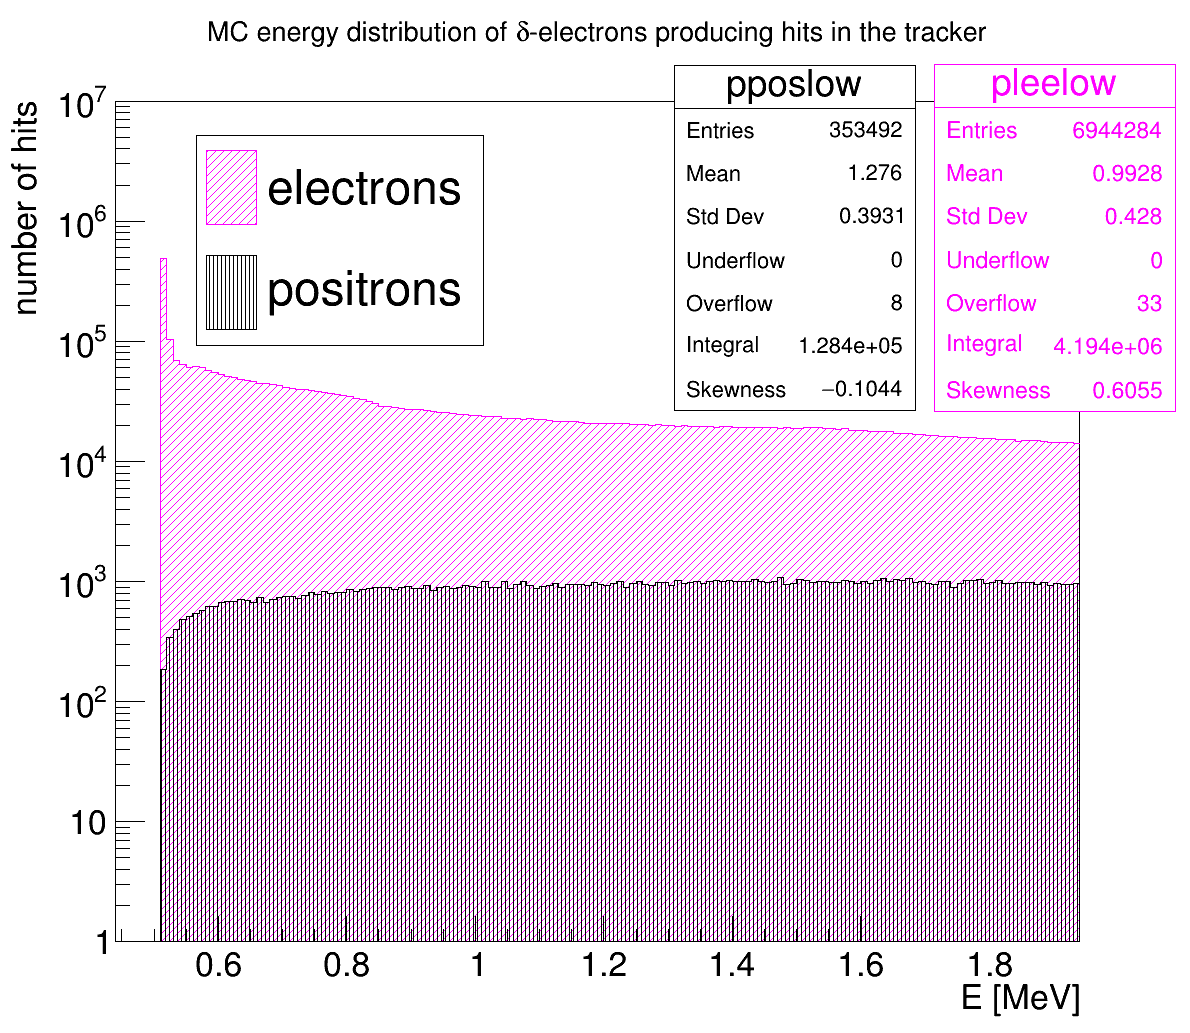
\includegraphics[width =0.7\textwidth]{figures/png/Screenshot_20240820_154854.png}
    \caption[The $\delta$-electrons energy distribution.]{The $\delta$-electrons energy distribution ($E<2$ MeV). Electrons 
    are shown in pink and positrons in black.}
    \label{fig:detail}
\end{figure}
For both the algorithms, another cause of failure 
in $\delta$ flagging arises from hits on straws that are 
parallel to each other, particularly those near the center of the tracker, 
with which stereo reconstruction is not possible. 

From both tables, it is also noticeable that the positron 
efficiency for $FlagBkgHits$ is lower compared to $DeltaFinder$. 
This is because the MVA output is statistics-dependent. In this 
energy range, positrons have very few $ComboHit$s, as 
they are not affected by Compton scattering. Therefore, 
$FlagBkgHits$ is less efficient with positrons for $E < 2$ MeV/c, 
but more efficient with electrons compared to 
$DeltaFinder$, due to the higher statistics.

For higher momentum values, both algorithms perform similarly and the 
differences between positrons and electrons become negligible.  
The sum of the positron and electron efficiency (Tables \ref{tab:2bbcele} 
and \ref{tab:1bbcele}) for a given algorithm 
matches that of the other algorithm, indicating they have the same 
capability in rejecting $\delta$-electrons. 

Figure \ref{fig:efficiency} shows that as the momentum 
increases, the efficiency decreases. This occurs because 
higher momenta correspond to larger radii and a 
greater spread of hits on the $x$-$y$ plane. 
This trend is also observed for particles in the 
next selected momentum range ($20 \ \text{MeV/c} <p<80 \ \text{MeV/c}$).


When comparing the two algorithms, especially in terms of 
CE flagging, there is a factor of 1.7 between the 
two $f_e$ values. The key difference lies in the following: 
CE hits can sometimes occur in close temporal and spatial 
proximity to other $\delta$ hits. Consequently, $FlagBkgHits$ 
flags these as $\delta$ hits because it does not attempt to 
correlate hits across different stations along the $z$-axis. 
In contrast, $DeltaFinder$ attempts to link $seed$s 
across stations, thereby distinguishing them more efficiently.

Concerning proton flagging, we could not compare the two 
algorithms since the $FlagBkgHits$, before creating $StereoHit$s, 
applies a preliminary selection cut on the energy deposited in 
the $StrawHit$s of 5 keV. Subsequently, the algorithm identifies 
protons as all particles with a deposited energy greater than 
4.5 keV. It was not possible to conduct a direct comparison, 
as $DeltaFinder$ does not apply a cut on the energy deposited in 
the $StrawHit$s, making the comparison unreliable and biased. 
Therefore, we reported the fraction of protons 
flagged as protons only by $DeltaFinder$.

From both Tables \ref{tab:2bbcele} and \ref{tab:1bbcele}, 
we observe that 3.7\% of 2BB and 2.5\% of 1BB low-momentum 
electron hits are misidentified as protons. These hits all have 
higher deposited energy. This occurs because energy loss depends 
on the particle's energy, which increases as the particle's energy 
decreases, leading to the misidentification. Positrons, however, 
are not affected by this misidentification, as they are not 
subject to Compton scattering and are not abundant in this energy range.


The results are comparable for both the 1BB and 2BB data samples.


    \begin{figure}[!h]
        \centering
        \begin{subfigure}[t]{0.5\textwidth}
            \centering
            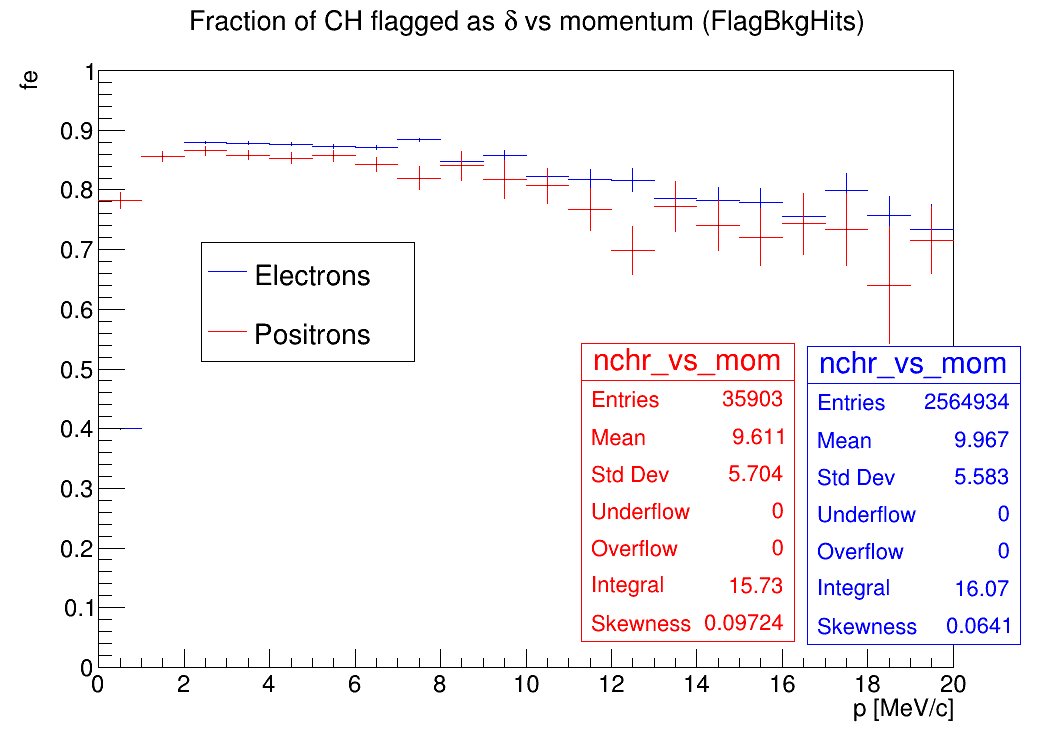
\includegraphics[width=1.\textwidth]{figures/png/Screenshot_20240818_155835.png}
            \caption{}
        \end{subfigure}%
        ~ 
        \begin{subfigure}[t]{0.5\textwidth}
            \centering
            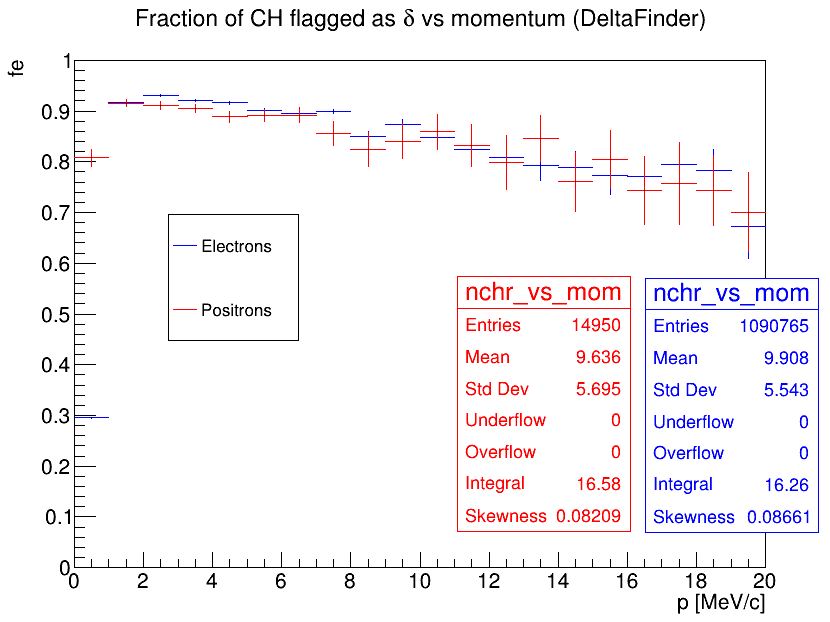
\includegraphics[width=0.95\textwidth]{figures/png/Screenshot_20240813_203916.png}
            \caption{}
        \end{subfigure}
        \caption[The efficiency of electrons and positrons versus 
        particle momentum in the low-momentum range.]{The efficiency of electrons (blue) and positrons (red) versus 
        particle momentum in the low-momentum range. The left plot shows the 
        results for $FlagBkgHits$, while the right plot shows those for $DeltaFinder$.
        }
        \label{fig:efficiency}
      \end{figure} 

      Looking at the results for $\mu$ and $\pi$ (Table \ref{tab:0bbpbar}), 
      we observe an approximate factor of 4 difference between the two algorithms 
      in muon flagging, and about a factor of 3.3 for pions 
      between the two algorithms. This occurs 
      because muons and pions often produce more than one hit in a single station, 
      but the $DeltaFinder$ algorithm is able to distinguish these hits, aided by 
      its ability to recognize straight lines in the $r-z$ plane, whereas 
      $FlagBkgHits$ cannot. Moreover, the problem with having a supervised 
      training method that distinguishes one type of particle (CE) from another ($\delta$-electrons)
      is that it can be confused when another type of particle, such as 
      tracks from $p\bar{p}$ annihilation, appears. 
      
      On average, pions from $p\bar{p}$ collisions have higher 
      momenta than muons, leading to a higher false positive rate. In fact, 
      there are more low-energy particles in the case of muons, making them 
      less likely to be correctly distinguished compared to pions. Furthermore, 
      the false positive rate ($f_p$) decreases as the momentum increases for pions, 
      according to the Bethe-Bloch formula.

    \begin{center}
        \begin{table}[h!]
        \centering
        \renewcommand{\arraystretch}{1.}
        \begin{tabular}{| c | c | c | c|} 
        \hline
         &  $f_{p}$ DF &  $f_{e}$ FBH & $f_{e}$ DF\\
        \hline
        $\mu$  &  2.7\%  & 13.0\% & 3.2\%\\
        \hline
        $\pi$ & 0.4\% & 23.8\%& 7.3\%\\
        \hline
        \end{tabular}
        \caption[Muon and Pion hit-level comparison.]{Muon and Pion 
        hit-level comparison ($PBAR-0BB$ data sample). FBH and DF denote 
        the $FlagBkgHits$ and $DeltaFinder$ algorithms respectively. $f_p$ and $f_e$ represent 
        the number of particle $ComboHit$s flagged as protons and electrons, respectively, 
        divided by the total number of $ComboHit$s.}
        \end{table}\label{tab:0bbpbar}
        \end{center}


\subsection{High-level comparison}
The unflagged hits are then passed to the pattern 
recognition algorithm, after which track reconstruction is performed. 
Figure \ref{fig:highlevel1} presents the momentum 
distribution of reconstructed tracks for the $CE-1BB$ 
data sample using both algorithms. 
In the case of $FlagBkgHits$ (blue), protons are not 
correctly flagged, resulting in their inclusion during 
pattern recognition and subsequent reconstruction. 
In contrast, $DeltaFinder$ (red) successfully flags 
proton hits, preventing them from entering the reconstruction stage. 
Figure \ref{fig:highlevel2} provides a zoomed-in view 
of the reconstructed track momentum distribution within 
the CE momentum range, where the reconstruction results 
from both algorithms are quite similar.

\begin{figure}[!h]
    \begin{subfigure}[b]{0.5\textwidth}
        \centering
        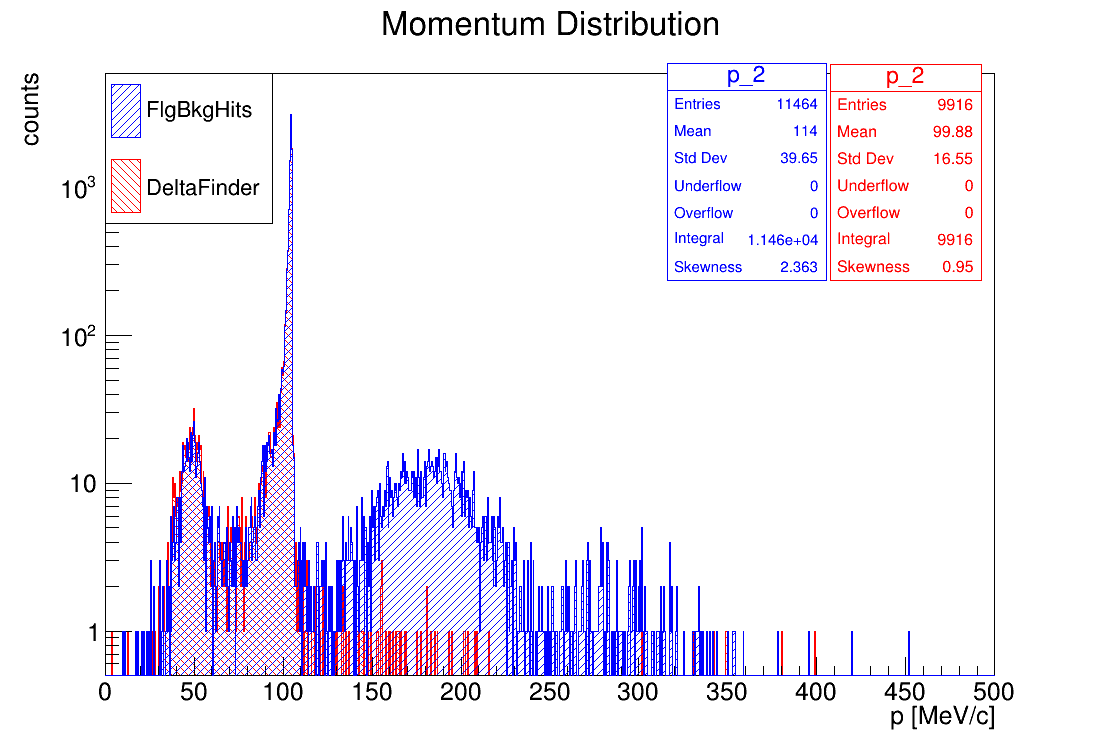
\includegraphics[width = 1.1\textwidth]{figures/png/Screenshot_20240820_162125.png}
        \subcaption{}
        \label{fig:highlevel1}
    \end{subfigure}
    \begin{subfigure}[b]{0.5\textwidth}
        \centering
        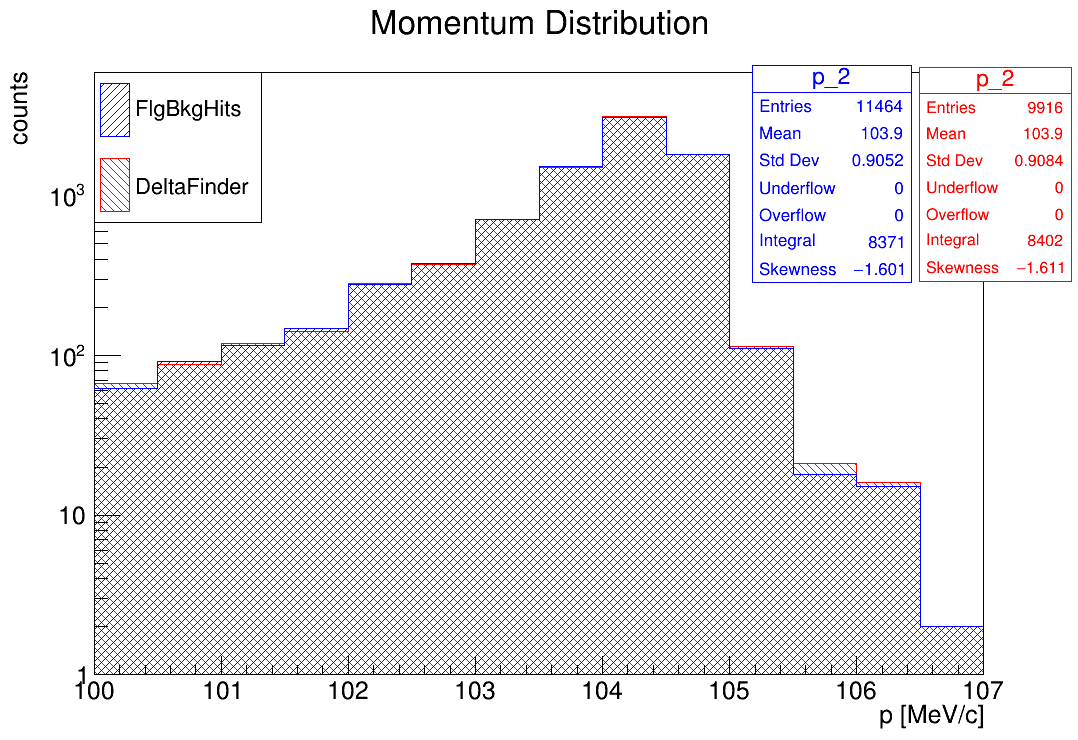
\includegraphics[width = 1.1\textwidth]{figures/png/Screenshot_20240820_160904.png}
        \subcaption{}
        \label{fig:highlevel2}
    \end{subfigure}
    \caption[Momentum distribution of reconstructed tracks.]{The momentum distribution of reconstructed tracks. 
    Tracks reconstructed using $FlagBkgHits$ as the $\delta$-flagger are shown in blue, while those 
    using $DeltaFinder$ are in red. The distribution in (a) covers a higher momentum range, while (b) 
    provides a zoomed-in view of the momentum range [100, 107] MeV/c.
    }
    \label{fig:highlevel} 
\end{figure}

The discrepancy in the number of reconstructed tracks, particularly 
for protons, is approximately 16\%, suggesting that $FlagBkgHits$ is 
capable of flagging only about one proton track every six events. 
Table \ref{tab:recoeffcele} reports the fraction of events associated 
with a true CE that have at least one reconstructed track (for both 2BB and 1BB). 
This fraction of CEs is nearly identical between the two algorithms, 
as expected from Figure \ref{fig:highlevel}. Table \ref{tab:1bbcele} shows 
that the difference in the number of hits between the two algorithms 
is less than one hit per track, which justifies the observed similarities in 
Table \ref{tab:recoeffcele}. The results are comparable for both 1BB and 2BB.



\begin{center}
    \begin{table}[h!]
    \centering
    \renewcommand{\arraystretch}{1.}
    \begin{tabular}{| c | c | c | c | c |} 
    \hline
    & FBH 2BB & DF 2BB & FBH 1BB & DF 1BB  \\
    \hline
    fraction of CE events with $N_{tracks}>0$ & 36.7\% & 36.5\% & 37.9\% & 37.9\%\\
    \hline
    \end{tabular}
    \caption[Fraction of reconstructed CE events.]{Fraction of reconstructed CE events ($CE-2BB$ and $CE-1BB$ data sample). FBH denotes 
    the $FlagBkgHits$ algorithm, and DF denotes the $DeltaFinder$ algorithm.}
    \end{table}\label{tab:recoeffcele}
\end{center}

To better understand the performance of the two algorithms, 
we analyzed events where at least one track was reconstructed 
using one hit flagger while no tracks were reconstructed 
with the other. A well defined class of events was identified in 
which the effects of hit flaggers are mitigated by the time 
clustering algorithm during reconstruction.

Figures \ref{fig:TZCluster1} ($FlagBkgHits$) and 
\ref{fig:TZCluster2} ($DeltaFinder$) illustrate the 
$time$ versus $z$ coordinate (aligned with the tracker) for 
the same event processed by both algorithms. In these plots, 
CE hits are represented by large red dots, $\delta$-electrons 
by small brown dots, and protons by large blue dots. Violet 
squares denote particles associated with the same $TimeCluster$, 
which is formed by grouping hits that align along a linear 
path in time versus $z$ space.
\begin{figure}[!h]
    \centering
    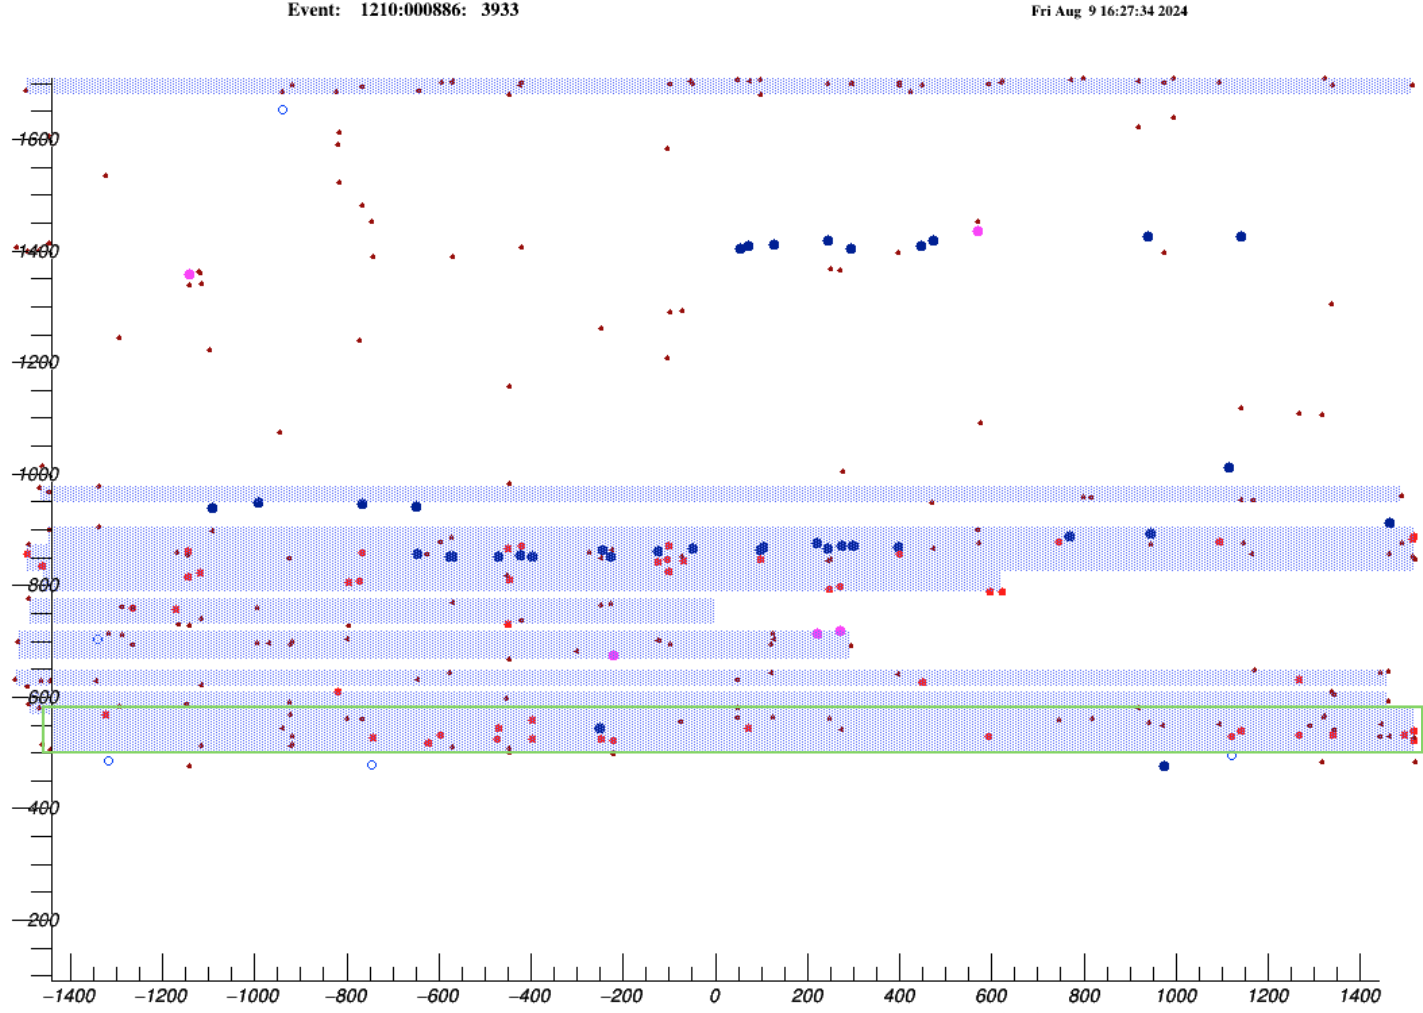
\includegraphics[width =0.7\textwidth]{figures/png/Screenshot_20240819_153229.png}
    \caption[$TimeCluster$ on $time-z$ plane.]{$TimeCluster$ (green) on $time-z$ plane. 
    This $TimeCluster$ is reconstructed using the $FlagBkgHits$ output.
    CE hits are represented by large red dots, $\delta$-electrons 
    by small brown dots, and protons by large blue dots. Violet 
    squares denote particles associated with the same $TimeCluster$.}
    \label{fig:TZCluster1}
\end{figure}
\begin{figure}[!h]
    \centering
    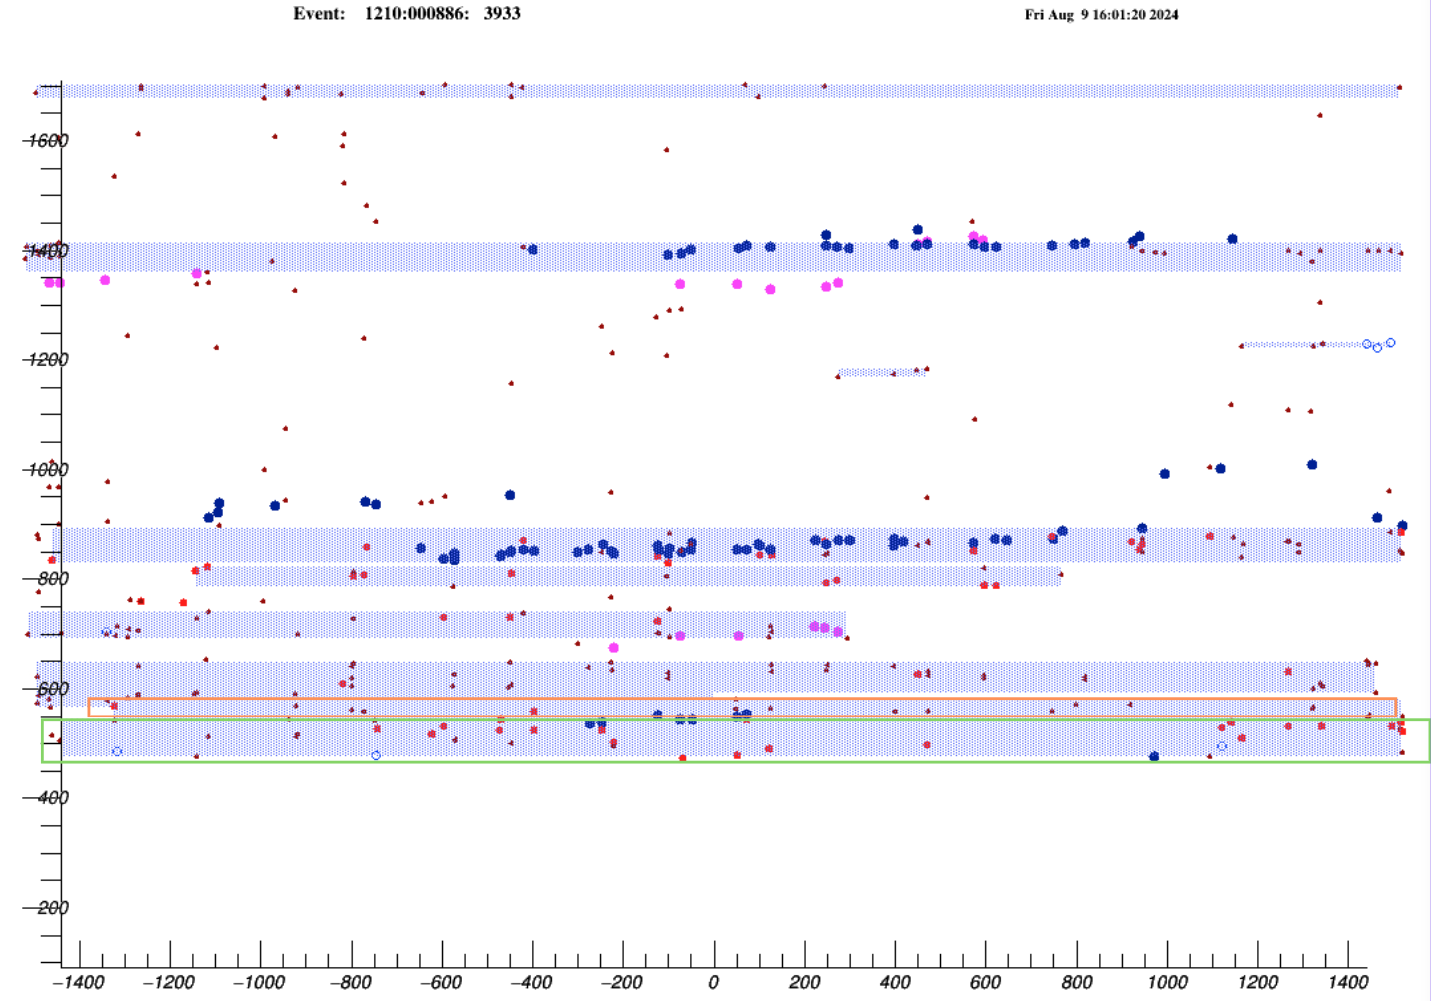
\includegraphics[width =0.7\textwidth]{figures/png/Screenshot_20240819_153730.png}
    \caption[$TimeCluster$ on $time-z$ plane.]{$TimeCluster$ (green and orange) on $time-z$ 
    plane. This $TimeCluster$ is reconstructed using the $DeltaFinder$ output.
    CE hits are the large red dots, $\delta$-electrons 
    the small brown ones, and protons the large blue ones. Violet 
    squares denote particles associated with the same $TimeCluster$.}
    \label{fig:TZCluster2}
\end{figure}
The time clustering process begins by combining hits within a specific $time-z$ 
window to create $chunks$ (with a 20 ns time window and a 5-plane z-window). 
A window qualifies as a $chunk$ if it contains more than three $ComboHit$s. 
Every potential pair of chunks within a certain time 
proximity is tested together, and the pair, that minimizes 
the $\chi^2/ndof$ when the hits are fit to a linear line, 
is combined. This procedure is repeated until no further combinations 
yield a $\chi^2/ndof$ below a set threshold. If a chunk 
exceeds a minimum number of straw hits, it is saved as a cluster.

Since particles grouped together may be at different $z$ values, 
$TimeCluster$s can exhibit varying $z$ coordinates. In Figure \ref{fig:TZCluster1}, 
all hits are grouped into a single cluster (green), 
while in Figure \ref{fig:TZCluster2} (green and orange), CE hits are divided into 
two different $TimeCluster$s.  
Specifically, in the $DeltaFinder$ algorithm, hits from the same 
particle are split into separate time clusters and no 
track are reconstructed. In contrast, with $FlagBkgHits$, 
unflagged hits are utilized by the time clusterer to $connect$ particle hits, 
leading to successful track reconstruction. 

This example highlights the importance of refining 
the cluster finder and pattern recognition algorithms to 
enhance track reconstruction performance.


Table \ref{tab:recoeffpbar} shows the fraction of events attributed 
to muons, pions, or electrons from $p\bar{p}$ annihilation, 
with at least two reconstructed tracks and using momentum cuts of 
either 80 MeV/c or 90 MeV/c. The 80 MeV/c cut represents the 
minimum particle momentum for which a particle can be reconstructed 
in Mu2e, due to acceptance limitations for particles originating from 
the stopping target. The 90 MeV/c cut is applied to ensure 
the complete elimination of DIO events. For Run I, requiring a 
DIO electron momentum above 90 MeV/c yields an estimate of 
approximately $10^{-2}$ events with two DIO electrons. With a 
track reconstruction efficiency of approximately 0.1, this corresponds 
to roughly $10^{-4}$ events with two DIO electron tracks. Assuming a 
uniform distribution in time, the number of such events within a 
100 ns window is approximately $10^{-5}$.

The $DeltaFinder$ algorithm demonstrates an advantage of 
approximately 22\% in reconstructing two tracks, attributed to 
its ability to distinguish between muon and pion hits compared to 
$\delta$-electrons (Table \ref{tab:0bbpbar}). The difference in 
hit-level efficiencies results in more than 12 hits per track difference 
between the two algorithms. After applying momentum cuts, the 
difference between the algorithms appears to be similar to that 
observed without a momentum cut.


\begin{center}
        \begin{table}[h!]
        \centering
        \renewcommand{\arraystretch}{1.}
        \begin{tabular}{| c | c | c |} 
            \hline
            &  FBH & DF\\
            \hline
            fraction of events with $N_{tracks} \geq 2$ &  1.8\% & 2.2\%\\
            \hline
            fraction of events with $N_{tracks} \geq 2$ \& $p>$80 MeV/c & 1.7\% & 2.1\%\\
            \hline
            fraction of events with $N_{tracks} \geq 2$ \& $p>$90 MeV/c & 1.6\% & 2.0\%\\
            \hline
            \end{tabular}
        \caption[Fraction of reconstructed $p\bar{p}$ events.]{Fraction of reconstructed $p\bar{p}$ events 
        ($PBAR-0BB$ data sample). FBH denotes the $FlagBkgHits$ algorithm, 
        and DF denotes the $DeltaFinder$ algorithm.}
        \end{table}\label{tab:recoeffpbar}
\end{center}

\section{Conclusions}
The Mu2e tracker will see approximately 75\% of its hit 
sources originate from $\delta$-electrons, which are electrons 
and positrons with momenta below 20 MeV/c. Two distinct algorithms 
have been developed in Mu2e Offline to identify these hits and exclude 
them from the reconstruction process: $FlagBkgHits$ and $DeltaFinder$. 
The $FlagBkgHits$ algorithm initially clusters the hits and then uses an ANN 
to classify them, while $DeltaFinder$ identifies clusters of hits that are 
consistent with those produced by low-momentum particles.

The performance of these two algorithms has been compared on two levels:

\begin{itemize}
    \item Hit-level comparison: it focuses on evaluating the 
    accuracy with which individual hits are flagged, providing a 
    direct method for comparing the algorithms' performance. In terms 
    of $\delta$-electron flagging, both algorithms perform similarly. 
    However, $DeltaFinder$ performs better in flagging positrons 
    due to the low statistics at energies below 2 MeV/c, 
    while this disadvantages $FlagBkgHits$ since the ANN is 
    statistics dependent, though it 
    performs worse with electrons as it struggles to reconstruct hits 
    that register only a single hit per station. Regarding CE hits, 
    $FlagBkgHits$ flags approximately 70\% more of these than 
    $DeltaFinder$, as it performs analysis on the $x$-$y$ plane and does 
    not reconstruct hits in the $z$ coordinate. Furthermore, 
    $DeltaFinder$ is capable of flagging proton hits (approximately 84\%), 
    a task that $FlagBkgHits$ cannot perform. It is crucial that hits 
    corresponding to $p\bar{p}$ annihilation are not flagged. This necessitates 
    examining muon and pion hit flagging, but $FlagBkgHits$ trained 
    on datasets lacking muon and pion hits and so 
    flags these particles at rates roughly 4 and 3.3 times higher, 
    respectively, than $DeltaFinder$.
    
    \item High-level comparison: This phase assesses the algorithms' 
    impact on subsequent stages of event reconstruction, particularly 
    how effectively each contributes to accurate track reconstruction. 
    The main observed difference between the two algorithms lies in the number 
    of reconstructed tracks using CE data samples, which is 16\% higher 
    for $FlagBkgHits$. This increase is due to $FlagBkgHits$ failing to 
    properly flag protons, allowing these particles to be sent to the 
    reconstruction stage. The difference in the reconstruction of 
    $p\bar{p}$ events, measured as the fraction of events with 
    at least two reconstructed tracks, is approximately 22\% higher with $DeltaFinder$.
\end{itemize}

Additionally, the processing time per event for each algorithm was 
monitored. For $FlagBkgHits$, it was necessary to account for the time 
spent creating the $StereoHit$s, while $DeltaFinder$ independently 
reconstructed the $seed$s. Processing $CE-1BB$ events required about 
0.14 ms/event for $FlagBkgHits$ plus an additional 0.15 ms/event, 
compared to 0.42 ms/event for $DeltaFinder$. For $CE-2BB$ events, 
$FlagBkgHits$ took approximately 0.37 ms/event plus 0.34 ms/event, 
while $DeltaFinder$ required 1.1 ms/event. Processing $PBAR-0BB$ 
events took about 0.02 ms/event plus 0.02 ms/event for $FlagBkgHits$, 
and 0.09 ms/event for $DeltaFinder$. The difference in processing time 
is negligible considering that the entire reconstruction process 
takes only a few ms per event.

The primary drawback of $FlagBkgHits$ is its reliance 
on supervised training using CE and $\delta$-electron samples. 
This approach fails when other particles, such as cosmic muons 
and those from $p\bar{p}$ annihilation, are introduced into the algorithm. 
Additionally, the training was performed using Monte Carlo data 
rather than real data, posing a potential risk when transitioning 
to actual data-taking. Moreover, being ANN-based, $FlagBkgHits$ 
performs poorly when the statistics are very low and lacks 
a well-defined method for proton flagging.
